%	Next lines is for compiling with arara package

%	First compiling: useful for generating .sxd files of the index
%	arara: pdflatex

%	Generate .sbx files of the index
%	arara: songidx: {input: ./chiesa}
%	arara: songidx: {input: ./party}
%	arara: songidx: {input: ./christmas}

%	Last compiling with complete indexes
%	arara: pdflatex


\documentclass[openright]{book}
%	Preamble
\usepackage[a5paper,left=15mm,right=15mm,bottom=10mm,top=15mm]{geometry}
\usepackage[utf8]{inputenc} % For special sybols
\usepackage{graphicx} % For pictures
\usepackage{latexsym} % For arrow
\usepackage{ulem} % For \xout
\usepackage{ifthen} % For if-then-else funtions
\usepackage[bookmarks]{hyperref} % For indexes

%	Header and footer
\usepackage{fancyhdr}
	\pagestyle{fancy}
%	\renewcommand{\chaptermark}[1]{\markboth{\textsc{#1}}{}}
	\fancyhf{}
	\fancyhead[LE,RO]{%\thepage
	}
	\fancyhead[RE,LO]{%\leftmark
	}
  \fancyhead[C]{%\leftmark
  }

%	Graphics of a license: use it at your own risk
%	\fancyfoot[C]{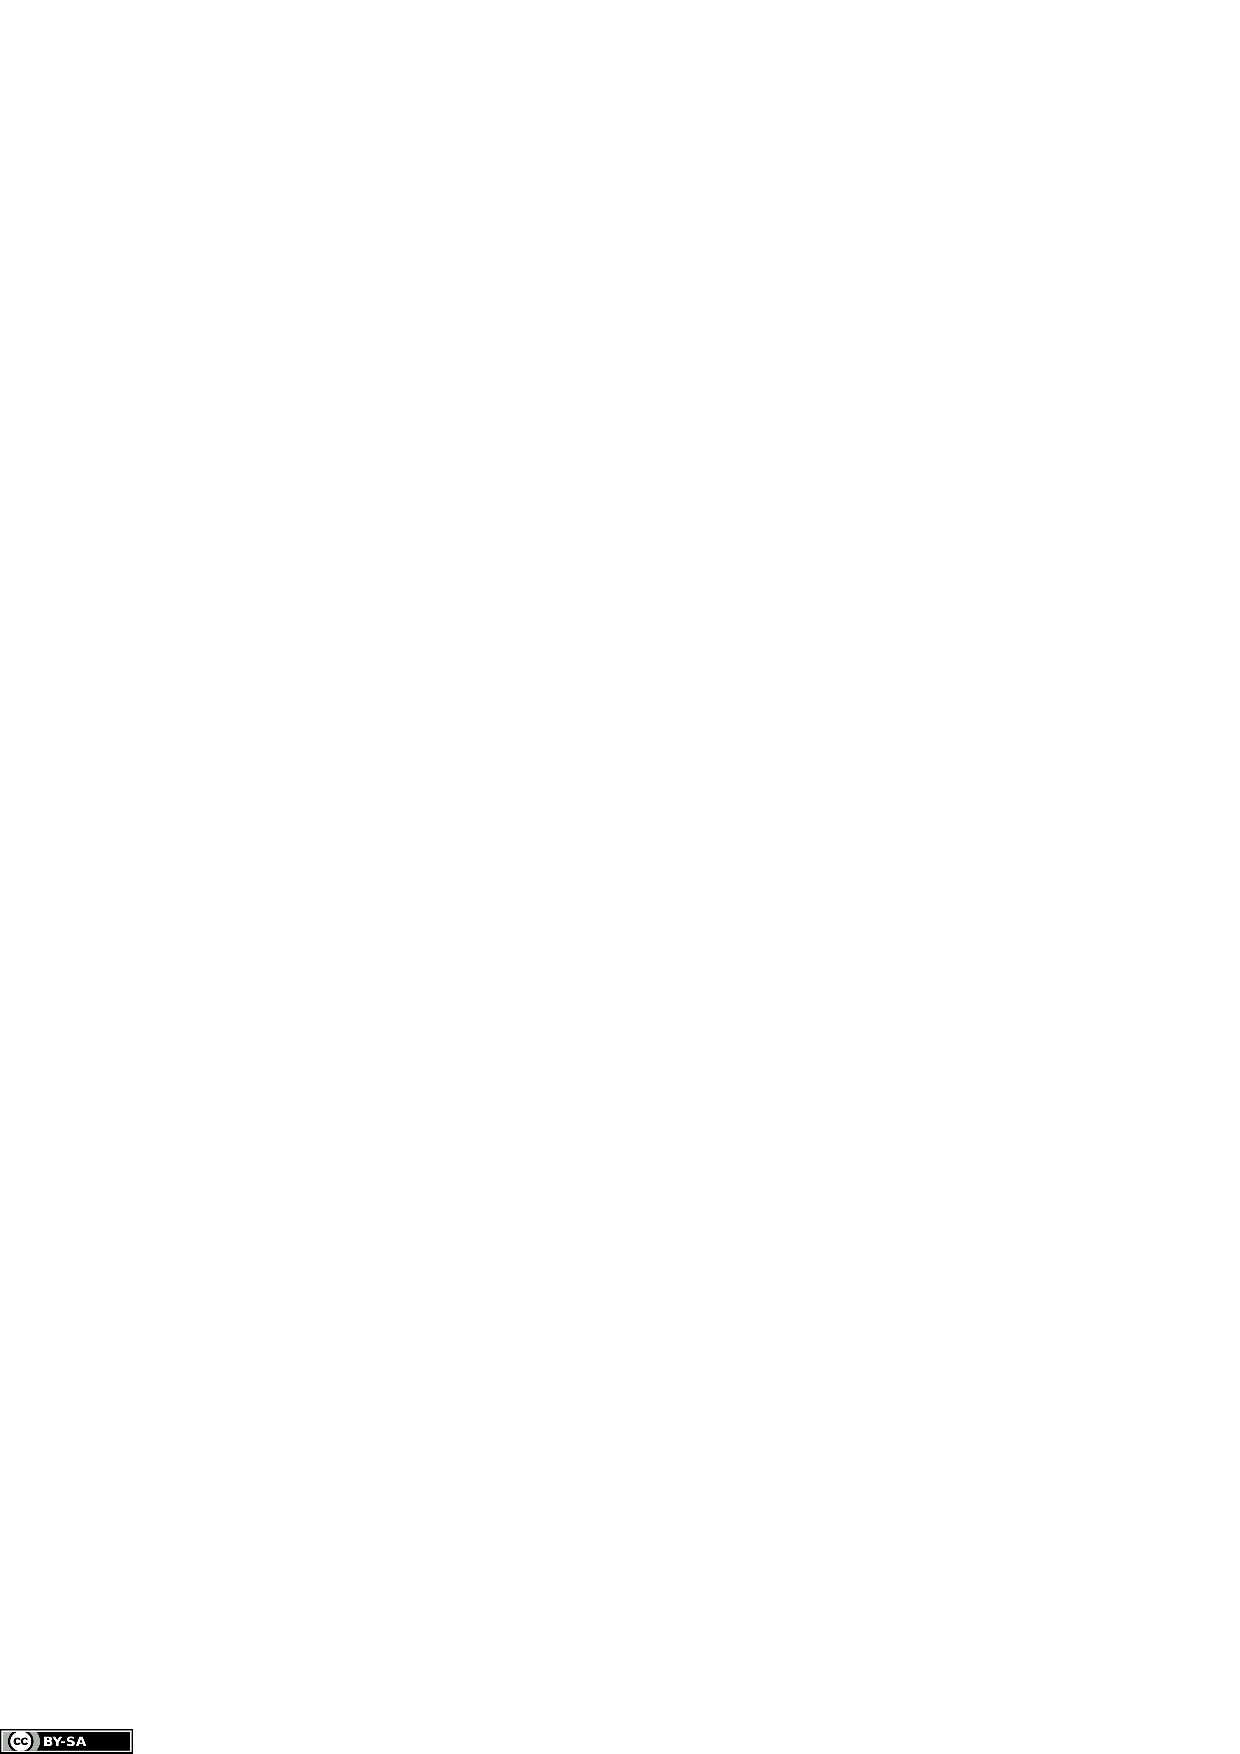
\includegraphics[]{img/cc-by-sa_80x15.png}}

	\renewcommand{\headrulewidth}{0pt}
	\renewcommand{\footrulewidth}{0pt}

%	Songs package and its parameters
\usepackage[chorded]{songs} % For chords book (xor with lyric)
%\usepackage[lyric]{songs} % For lyrics book (xor with chorded)
	\nosongnumbers
	%\noversenumbers
	%\includeonlysongs{37,50,2}
	\prefersharps % For automatic transpositions

%	Indexes
	\newindex{chiesa}{chiesa}
	\newindex{party}{party}
	\newindex{christmas}{christmas}

%	Fonts
	\renewcommand{\lyricfont}{\sffamily}
	\renewcommand{\printchord}[1]{\rmfamily\bf#1}

	\songcolumns{1} % Number of columns for every page

%	Page-breanking and column-breaking
	\spenalty=-10000	% At song boundaries (-10000: the break is required)
%	\brkpenalty=200		% Wherever \brk is used
%	\vvpenalty=50 		% Verse to verse breaking
%	\ccpenalty=50 		% Chorus to chorus breaking
%	\vcpenalty=50 		% Verse to chorus breaking
%	\cvpenalty=50 		% Chorus to Verse breaking

  \songpos{3} % Aggressiveness of song-positioning algorithm

%	The width of the shaded boxes that begin each alphabetic block of a large title index
%	\setlength{\idxheadwidth}{1cm}

%	\sepindexesfalse
%	\sepindexestrue
%	\songtarget
%	\songlink


%	Formatting: if the page is even, add a black page before.
%	(Useful to format the start of a chapter)
\newcommand{\checkodd}{
	\ifthenelse{\isodd{\thepage}}{
		%if page is odd: ok
	}{
		%else: page is even: add a page before
		\vspace*{\fill}
		\clearpage
	}
}
%	Formatting: if the page is odd, add a black page before.
%	(Useful to format the end of the book)
\newcommand{\checkeven}{
	\ifthenelse{\isodd{\thepage}}{
		%page is odd: add a page before
		\vspace*{\fill}
		\clearpage
	}{
		%else: page is even: ok
	}
}

%	Localization: remove the autogenerated files before changing the locales

\usepackage[italian]{babel} % For italian language

%	For italian notation: parameters of songs package (put it after the declaration of that package)
  \notenamesin{A}{B}{C}{D}{E}{F}{G}  
  \notenamesout{LA}{SI}{DO}{RE}{MI}{FA}{SOL}
 % Italian locale

%	Begin the book
\begin{document}


\begin{titlepage}
	\centering
	\vspace*{\stretch{6}}
	{\sffamily\huge\bfseries GuitarHub\par}
	\vspace*{\stretch{1}}
	{\ttfamily\scshape\Large Chords and Lyrics Book\par}
	\vspace*{\stretch{8}}
	
\includegraphics[scale=0.3]{img/GitHub-Mark-64px}\par % GitHub picture
	{\ttfamily\footnotesize https://github.com/PietroPrandini/GuitarHub\par}
%	Set license: use it at your own risk
%	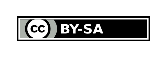
\includegraphics[]{img/cc-by-sa_80x15}
	\vspace*{\stretch{3}}
\end{titlepage}

 % Front page

%	Set license: use it at your own risk
% English license
%\vspace*{\fill}
%\begin{center}
%	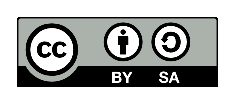
\includegraphics[]{img/cc-by-sa_88x31}
%\end{center} \par
%This work is licensed under the Creative Commons Attribution-ShareAlike 4.0 International License. To view a copy of this license, visit http://creativecommons.org/licenses/by-sa/4.0/ or send a letter to Creative Commons, PO Box 1866, Mountain View, CA 94042, USA. \par
%\pagebreak

%	Set license: use it at your own risk
% Italian license
%\vspace*{\fill}
%\begin{center}
%	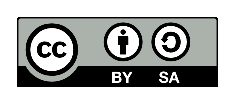
\includegraphics[]{img/cc-by-sa_88x31}
%\end{center} \par
%Quest'opera \`e stata rilasciata con licenza Creative Commons Attribuzione - Condividi allo stesso modo 4.0 Internazionale. Per leggere una copia della licenza visita il sito web http://creativecommons.org/licenses/by-sa/4.0/ o spedisci una lettera a Creative Commons, PO Box 1866, Mountain View, CA 94042, USA. \par
%\pagebreak

%	Showing indexes
\showindex[2]{Canti per la Liturgia, per le Celebrazioni e per la Preghiera}{chiesa}
\showindex[2]{Party}{party}
\showindex[2]{Christmas}{christmas}

% New chapter
% Start on a right page and the title is in a blank page
\checkodd
\vspace*{\stretch{3}}
\songchapter{Canti per la Liturgia, per le Celebrazioni e per la Preghiera}
\vspace*{\stretch{5}}
\newpage
% Songs of this chapter
\begin{songs}{chiesa}
	%	Songs of the chiesa chapter
\input{"tex/chiesa/Adoro Te"}
\beginsong{Alleluia questa Tua parola}[
,cr={\centering{\href{https://github.com/PietroPrandini/GuitarHub}{https://github.com/PietroPrandini/GuitarHub} - \href{http://creativecommons.org/licenses/by-sa/4.0/}{CC-BY-SA} - \filemodprintdate{"tex/chiesa/Alleluia questa Tua parola.tex"}}}, % Copyright information
]
\transpose{0}
%{\nolyrics Intro: }

\ifchorded
\beginverse*
{\nolyrics Intro: \[D] \[Em] \[G] \[D]}
\endverse
\fi

\beginchorus
\[D]Alleluia, \[A]Alleluia, \[Bm]Alleluia, A\[F#]lleluia,
\[G]Alleluia, \[D]Alleluia, \[E]Alleluia, A\[A4]lle\[A]luia.
\[D]Alleluia, \[A]Alleluia, \[Bm]Alleluia, A\[F#]lleluia,
\[G]Alleluia, \[D]Alleluia, \[E]Alleluia, A\[A4]lle\[A]lui\[D]a.
\endchorus

\beginverse*
\[D]Questa Tua parola \[C]non avr\`a mai fine,
\[G]ha varcato i cieli e \[D]porter\`a i suoi frutti.
\[D]Questa Tua parola \[C]non avr\`a mai fine,
\[G]ha varcato i cieli e \[A4]porter\`a i suoi \[A7]frutti.
\endverse

\beginchorus
\[D]Alleluia, \[A]Alleluia, \[Bm]Alleluia, A\[F#]lleluia,
\[G]Alleluia, \[D]Alleluia, \[E]Alleluia, A\[A4]lle\[A]lui\[D]a.
\endchorus

\endsong

\beginsong{%Titles
Benedici o Signore}[
%by={},%authors, composers, and other contributors
,cr={\centering{\href{https://github.com/PietroPrandini/GuitarHub}{https://github.com/PietroPrandini/GuitarHub} - \href{http://creativecommons.org/licenses/by-sa/4.0/}{CC-BY-SA} - \filemodprintdate{"tex/songsBodies/Benedici o Signore.tex"}}}, % Copyright information
%sr={},%related scripture references
%index={},%an extra index entry for a line of lyrics
%ititle={}%an extra index entry for a hidden title
]

%\capo{0}
\transpose{0}

\beginsong{%Titles
Benedici o Signore}[
%by={},%authors, composers, and other contributors
,cr={\centering{\href{https://github.com/PietroPrandini/GuitarHub}{https://github.com/PietroPrandini/GuitarHub} - \href{http://creativecommons.org/licenses/by-sa/4.0/}{CC-BY-SA} - \filemodprintdate{"tex/songsBodies/Benedici o Signore.tex"}}}, % Copyright information
%sr={},%related scripture references
%index={},%an extra index entry for a line of lyrics
%ititle={}%an extra index entry for a hidden title
]

%\capo{0}
\transpose{0}

\input{"tex/songsBodies/Benedici o Signore.tex"}

\endsong


\endsong

\beginsong{%Titles
Benedici o Signore
}[
%by={},%authors, composers, and other contributors
%cr={},%copyright information
%li={},%licensing information
%sr={},%related scripture references
%index={V1},%an extra index entry for a line of lyrics
%ititle={V1}%an extra index entry for a hidden title
]

\capo{1}
\transpose{9}

\ifchorded
  \beginverse* % * not count the verse
	  {\nolyrics Intro: \[Dm] \[C] \[B&] \[A]}
  \endverse
\fi
	\beginverse\memorize % \memorize is used to set the chords you would like to use with ^ in the next verses
	%verse
	\[Dm]Nebbia e freddo, giorni lunghi e \[C]amari,
	mentre il seme m\[Dm]uore.
	\[F]Poi il prodigio, antico e sempre \[C]nuovo
	del primo filo d'\[B&]erba... e nel \[F]vento
	dell'es\[C]tate ond\[Dm]eggiano le \[F]spighe:
	a\[C]vremo ancora \[A]pan\[D]e!
	\endverse

	\beginchorus
	%chorus
	\[G]Bened\[D]ici, \[G]o \[D]Signore \[C]questa o\[G]fferta
	che por\[A]tiamo a Te.
	\[G]Facci \[D]uno, \[Bm]come il \[F#m]Pane \[E]che anche \[G]oggi
	hai \[D]dato a noi.
	\endchorus
	
	\beginverse
	^Nei filari, dopo il lungo ^inverno,
	fremono le ^viti.
	^La rugiada avvolge nel si^lenzio
	i primi tralci ^verdi... Poi i ^colori
	dell'aut^unno, coi ^grappoli ^maturi:
	a^vremo ancora ^vi^no! 
	\endverse
% \textnote{} %for notes

%                 Do     Re     Mi     Fa     Sol    La     Si
%Naturali:        \[C]   \[D]   \[E]   \[F]   \[G]   \[A]   \[B]
%Bemolli:         \[C&]  \[D&]  \[E&]  \[F&]  \[G&]  \[A&]  \[B&]
%Diesis:          \[C#]  \[D#]  \[E#]  \[F#]  \[G#]  \[A#]  \[B#]
%Minori:          \[Cm]  \[Dm]  \[Em]  \[Fm]  \[Gm]  \[Am]  \[Bm]
%Bemolli minori:  \[C&m] \[D&m] \[E&m] \[F&m] \[G&m] \[A&m] \[B&m]
%Diesis minori:   \[C#m] \[D#m] \[E#m] \[F#m] \[G#m] \[A#m] \[B#m]

\endsong

% Copyright 2018-2021 Pietro Prandini
% 
% This file is part of GuitarHub.
% 
% GuitarHub is free software: you can redistribute it and/or modify
% it under the terms of the GNU General Public License as published by
% the Free Software Foundation, either version 3 of the License, or
% (at your option) any later version.
% 
% GuitarHub is distributed in the hope that it will be useful,
% but WITHOUT ANY WARRANTY; without even the implied warranty of
% MERCHANTABILITY or FITNESS FOR A PARTICULAR PURPOSE.  See the
% GNU General Public License for more details.
% 
% You should have received a copy of the GNU General Public License
% along with GuitarHub.  If not, see <https://www.gnu.org/licenses/>.

\ifchorded

  \beginverse* 
{\nolyrics Intro: \[E] \[G#m] \[A] \[B] \rep{2}}
  \endverse

\fi

\beginverse\memorize 
\[A]Tu ci raduni da ogni \[E]parte del mondo
noi si\[F#m]amo tuoi figli, tuo \[C#m]popolo san\[B]to.
\[A]Lodiamo in coro con le \[B]schiere ce\[C#m]lesti,
in\[D]sieme cantiamo, gio\[A]iosi accla\[B]miamo.
\endverse

\beginchorus
\[E]O Si\[B]gnore, ve\[A]niamo a \[B]Te,
    \[E]con i c\[B]uori ri\[A]colmi di \[A&]gioia,
    \[A]Ti \[B]ringraziamo per i \[F#m]doni che \[C#m]dai
    \[A]e per l'\[B]amore che riv\[F#m]ersi in no\[B]i.
    \[E]O Si\[B]gnore, ve\[A]niamo a \[A]Te,
    \[E]con i c\[B]uori ri\[A]colmi di \[A&]gioia,
    \[C#m]le nostre \[A&m]mani inna\[F#m]lziamo al \[C#m]cielo,
    \[A]a te con \[B]gioia ven\[E]iam. \[G#m] \[A] \[B]
  \endchorus

  \textnote{Ending: a te con gioia veniam (x3)}
\beginverse
  ^La Parola che ci ^doni Signore,
  ill^umina i cuori, ci ^mostra la ^via.
  ^Dove andremo se non ^resti con ^noi?
  Tu ^solo sei vita, ^tu sei veri^t\`a.
\endverse

\beginverse
^La grazia immensa che ci ^doni Signore
pur^ifica i cuori, con^sola i tuoi fi^gli.
^Nel tuo nome noi ^speriamo ^Signore
sal^vezza del mondo, ^eterno splen^dore.
\endverse


\beginsong{Con gioia veniamo a Te}[
%by={authors, composers, and other contributors},
,cr={\centering{\href{https://github.com/PietroPrandini/GuitarHub}{https://github.com/PietroPrandini/GuitarHub} \href{http://creativecommons.org/licenses/by-sa/4.0/}{CC-BY-SA} \filemodprintdate{"tex/chiesa/Con gioia veniamo a te -2.tex"}}}, % Copyright information
%li={licensing information},
%sr={related scripture references},
%index={an extra index entry for a line of lyrics},
%ititle={an extra index entry for a hidden title}
]

%\capo{0}
\transpose{10}

\ifchorded
  \beginverse* % * not count the verse
		{\nolyrics Intro: \[E] \[G#m] \[A] \[B] \rep{2}}
  \endverse
\fi
	\beginverse\memorize % \memorize is used to set the chords you would like to use with ^ in the next verses
		\[A]Tu ci raduni da ogni \[E]parte del mondo
		noi si\[F#m]amo tuoi figli, tuo \[C#m]popolo san\[B]to.
		\[A]Lodiamo in coro con le \[B]schiere ce\[C#m]lesti,
		in\[D]sieme cantiamo, gio\[A]iosi accla\[B]miamo.
	\endverse

	\beginchorus
		\[E]O Si\[B]gnore, ve\[A]niamo a \[B]Te,
    \[E]con i c\[B]uori ri\[A]colmi di \[A&]gioia,
    \[A]Ti \[B]ringraziamo per i \[F#m]doni che \[C#m]dai
    \[A]e per l'\[B]amore che riv\[F#m]ersi in no\[B]i.
    \[E]O Si\[B]gnore, ve\[A]niamo a \[A]Te,
    \[E]con i c\[B]uori ri\[A]colmi di \[A&]gioia,
    \[C#m]le nostre \[A&m]mani inna\[F#m]lziamo al \[C#m]cielo,
    \[A]a te con \[B]gioia ven\[E]iam. \[G#m] \[A] \[B]
  \endchorus
  \textnote{Ending: a te con gioia veniam (x3)}

	\beginverse
	  ^La Parola che ci ^doni Signore,
	  ill^umina i cuori, ci ^mostra la ^via.
	  ^Dove andremo se non ^resti con ^noi?
	  Tu ^solo sei vita, ^tu sei veri^t\`a.
	\endverse

	\beginverse
		^La grazia immensa che ci ^doni Signore
		pur^ifica i cuori, con^sola i tuoi fi^gli.
		^Nel tuo nome noi ^speriamo ^Signore
		sal^vezza del mondo, ^eterno splen^dore.
	\endverse

% \textnote{} %for notes

%                 Do     Re     Mi     Fa     Sol    La     Si
%Naturali:        \[C]   \[D]   \[E]   \[F]   \[G]   \[A]   \[B]
%Bemolli:         \[C&]  \[D&]  \[E&]  \[F&]  \[G&]  \[A&]  \[B&]
%Diesis:          \[C#]  \[D#]  \[E#]  \[F#]  \[G#]  \[A#]  \[B#]
%Minori:          \[Cm]  \[Dm]  \[Em]  \[Fm]  \[Gm]  \[Am]  \[Bm]
%Bemolli minori:  \[C&m] \[D&m] \[E&m] \[F&m] \[G&m] \[A&m] \[B&m]
%Diesis minori:   \[C#m] \[D#m] \[E#m] \[F#m] \[G#m] \[A#m] \[B#m]

\endsong

% Copyright 2018-2024 Pietro Prandini
% 
% This file is part of GuitarHub.
% 
% GuitarHub is free software: you can redistribute it and/or modify
% it under the terms of the GNU General Public License as published by
% the Free Software Foundation, either version 3 of the License, or
% (at your option) any later version.
% 
% GuitarHub is distributed in the hope that it will be useful,
% but WITHOUT ANY WARRANTY; without even the implied warranty of
% MERCHANTABILITY or FITNESS FOR A PARTICULAR PURPOSE.  See the
% GNU General Public License for more details.
% 
% You should have received a copy of the GNU General Public License
% along with GuitarHub.  If not, see <https://www.gnu.org/licenses/>.

\ifchorded

\beginverse* 
{\nolyrics Intro: \[A] \[Bm] \[F#m] \[G] \[D] \[Em] \[D]}
\endverse

\fi

\beginchorus
\[D]Del tuo \[G]Spiri\[D]to, \[G]Signo\[D]re, \[A]\'e \[Bm]piena la \[F#m]terr\[G]a,
\'e \[D]piena la \[Em]terr\[D]a. \rep{2}
\endchorus

\beginverse\memorize
\[C]Benedici il Si\[B&]gnore,
\[Dm]anima \[Am]mi\[B&]a,
Si\[C]gnore, \[F]Dio\[C],
tu sei \[G]grand\[C]e!
\[C]Sono immense, splend\[B&]enti
\[Dm]tutte le Tue o\[B&]per\[F]e
e t\[Gm]utte le crea\[Gm]tur\[D]e.
\endverse

\beginverse
^Se tu togli il tuo ^soffio
^muore ogni ^cos^a
e ^si diss^olv^e
nella ^terr^a.
^Il tuo spirito ^scende
^tutto si ^ricre^a
e t^utto si ^rinnov^a.
\endverse

\beginverse
^La tua gloria, Si^gnore,
^resti per ^sempr^e.
Gio^isci, ^Di^o,
del cr^eat^o.
^Questo semplice ^canto
^salga a te Si^gnor^e
sei ^tu la nostra gi^oi^a.
\endverse


\beginsong{%Titles
\`E giunta l'ora}[
%by={}%authors, composers, and other contributors
%,cr={}%copyright information
%,li={}%licensing information
%,sr={}%related scripture references
%,index={}%an extra index entry for a line of lyrics
%,ititle={}%an extra index entry for a hidden title
]

%\capo{0}
\transpose{0}

%	\beginverse* % * not count the verse
%		{\nolyrics Intro: }
%	\endverse

%	\beginverse\memorize % \memorize is used to set the chords you would like to use with ^ in the next verses
		%verse
%	\endverse

%	\beginchorus
		%chorus
%	\endchorus

\beginverse\memorize
\`E giunta \[F]l’ora, \[B&]Padre, per \[F]me:
ai miei a\[Dm]mici \[B&] ho detto \[Gm]che \[C]
questa \`e la \[Am]vita: \[Dm]conoscere \[Am]Te
e \[B&]il Figlio \[C]Tuo: Cristo Ge\[F]s\`u. \[B&]\[F]
\endverse
\beginverse
Erano ^tuoi, ^li hai dati a ^me,
ed ora ^sanno ^che torno a ^Te.^
Hanno cre^duto: ^conservali ^Tu
nel ^tuo Am^ore, nell’uni^t\`a. ^^
\endverse
\beginverse
Tu mi hai ^mandato ^ai figli ^tuoi:
la tua ^parola ^\`e veri^t\`a.^
E il loro ^cuore ^sia pieno di gi^oia:
la ^gioia ^vera viene da ^Te.^^
\endverse
\beginverse
Io sono in ^loro e ^Tu in ^me;
e siam ^perfetti ^nell’uni^t\`a;^
e il mondo ^creda ^che Tu mi hai mand^ato:
li ^hai am^ati come ami ^me.^^
\endverse

%	\textnote{} %for notes

%                 Do     Re     Mi     Fa     Sol    La     Si
%Naturali:        \[C]   \[D]   \[E]   \[F]   \[G]   \[A]   \[B]
%Bemolli:         \[C&]  \[D&]  \[E&]  \[F&]  \[G&]  \[A&]  \[B&]
%Diesis:          \[C#]  \[D#]  \[E#]  \[F#]  \[G#]  \[A#]  \[B#]
%Minori:          \[Cm]  \[Dm]  \[Em]  \[Fm]  \[Gm]  \[Am]  \[Bm]
%Bemolli minori:  \[C&m] \[D&m] \[E&m] \[F&m] \[G&m] \[A&m] \[B&m]
%Diesis minori:   \[C#m] \[D#m] \[E#m] \[F#m] \[G#m] \[A#m] \[B#m]

\endsong

\beginsong{\`E Natale}[
by={Forza venite gente}
,cr={\centering{\href{https://github.com/PietroPrandini/GuitarHub}{https://github.com/PietroPrandini/GuitarHub}\\\href{http://creativecommons.org/licenses/by-sa/4.0/}{\textbf{CC BY-SA}} Pietro Prandini 2021}}, % Copyright information
%sr={related scripture references},
%index={an extra index entry for a line of lyrics},
%ititle={an extra index entry for a hidden title}
]
\transpose{0}

\beginsong{\`E Natale}[
by={Forza venite gente}
,cr={\centering{\href{https://github.com/PietroPrandini/GuitarHub}{https://github.com/PietroPrandini/GuitarHub}\\\href{http://creativecommons.org/licenses/by-sa/4.0/}{\textbf{CC BY-SA}} Pietro Prandini 2021}}, % Copyright information
%sr={related scripture references},
%index={an extra index entry for a line of lyrics},
%ititle={an extra index entry for a hidden title}
]
\transpose{0}

\input{"tex/songs/E Natale.tex"}

\endsong


\endsong

\beginsong{\`E Natale}[
by={Forza venite gente},
,cr={\centering{\href{https://github.com/PietroPrandini/GuitarHub}{https://github.com/PietroPrandini/GuitarHub} - \href{http://creativecommons.org/licenses/by-sa/4.0/}{CC-BY-SA} - \filemodprintdate{"tex/songsBodies/E Natale.tex"}}}, % Copyright information
%sr={related scripture references},
%index={an extra index entry for a line of lyrics},
%ititle={an extra index entry for a hidden title}
]
\transpose{10}

\beginsong{\`E Natale}[
by={Forza venite gente}
,cr={\centering{\href{https://github.com/PietroPrandini/GuitarHub}{https://github.com/PietroPrandini/GuitarHub}\\\href{http://creativecommons.org/licenses/by-sa/4.0/}{\textbf{CC BY-SA}} Pietro Prandini 2021}}, % Copyright information
%sr={related scripture references},
%index={an extra index entry for a line of lyrics},
%ititle={an extra index entry for a hidden title}
]
\transpose{0}

\input{"tex/songs/E Natale.tex"}

\endsong


\endsong

% Copyright 2018-2023 Pietro Prandini
% 
% This file is part of GuitarHub.
% 
% GuitarHub is free software: you can redistribute it and/or modify
% it under the terms of the GNU General Public License as published by
% the Free Software Foundation, either version 3 of the License, or
% (at your option) any later version.
% 
% GuitarHub is distributed in the hope that it will be useful,
% but WITHOUT ANY WARRANTY; without even the implied warranty of
% MERCHANTABILITY or FITNESS FOR A PARTICULAR PURPOSE.  See the
% GNU General Public License for more details.
% 
% You should have received a copy of the GNU General Public License
% along with GuitarHub.  If not, see <https://www.gnu.org/licenses/>.

\ifchorded

  \beginverse* 
  {\nolyrics Intro: \[C] \[B&] \[F] \[C7] x2}
  \endverse

\fi

\beginverse\memorize 
\[C]Scende il cielo sulla terra
sopra l'odio e sulla guerra
\[C7]scende il cielo e si fa storia
\[F]sfida il tempo e la memoria
\[C]ora \`e \[F] Natale an\[C]cora.
\endverse

\beginverse*
^Il passato \`e nel presente
nel futuro della gente
^e la pace \`e sempre un sogno
^dell'amore si ha bisogno
^ora \`e ^ Natale an^cora.
\endverse

\beginverse*
\[G]Ogni uomo pu\`o sentire
\[F]un segnale da seguire
\[C]ora \`e \[F] Natale an\[C]cora.
\endverse

\beginverse*
\[G]Ogni uomo qui nel mondo
\[F]una stella sta cercando
\[Dm]una luce \[Em]per torvare \[F]un po' di veri\[G]t\`a.
\endverse

\beginchorus
\[C]Merry Christmas all over the \[C7]world
\[F]nous chantons c'est Noel pour le \[Dm]monde
\[Am]buon Natale feliz \[Em]Navidad
\[F]per la pace \[Dm]che un giorno verr\`a\[G].
\[C]Merry Christmas all over the \[C7]world
\[F]c'est Noel non scordiamolo \[Dm]mai
\[Am]buon Natale feliz \[Em]Navidad
\[Fm]e la pace \[Dm]sia sempre con \[G]noi.
\ifchorded

  {\nolyrics \[C] \[B&] \[F] \[C7] \rep{2}}
\fi

\endchorus

  \beginverse
  \[C]Siamo popoli e nazioni
  secoli e generazioni
  \[C7]siamo figli del creato
  \[F]del presente e del passato
\[C]ora \`e \[F] Natale an\[C]cora.
  \endverse

  \beginverse*
  \[G]Nelle mani le bandiere
  \[F]nei paesi le frotiere
  \[Dm]ma nel cielo \[Em]il grido forte \[F]della liber\[G]t\`a.
  \endverse


% Copyright 2018-2021 Pietro Prandini
% 
% This file is part of GuitarHub.
% 
% GuitarHub is free software: you can redistribute it and/or modify
% it under the terms of the GNU General Public License as published by
% the Free Software Foundation, either version 3 of the License, or
% (at your option) any later version.
% 
% GuitarHub is distributed in the hope that it will be useful,
% but WITHOUT ANY WARRANTY; without even the implied warranty of
% MERCHANTABILITY or FITNESS FOR A PARTICULAR PURPOSE.  See the
% GNU General Public License for more details.
% 
% You should have received a copy of the GNU General Public License
% along with GuitarHub.  If not, see <https://www.gnu.org/licenses/>.

\beginverse\memorize 
\[D]Io lo so, Si\[F#m]gnore, che ve\[G]ngo da lon\[D]tano,
\[D]prima del pen\[F#m]siero e \[G]poi nella Tua m\[A]ano,
\[D]io mi rendo c\[A]onto che \[G]Tu sei la mia v\[D]ita
e \[G]non mi sembra \[Em]vero di preg\[E7]arti co\[A7]s\`i.
\endverse

\beginverse*
^"Padre d'ogni u^omo" e ^non Ti ho visto m^ai,
^"Spirito di ^vita" e ^nacqui da una don^na,
^"Figlio mio fra^tello" e ^sono solo un u^omo,
epp^ure io ca^pisco che ^Tu sei Ve^rit\`a.
\endverse

\beginchorus
E im\[D]parer\`o a gu\[G]ardare tutto \[A7]il mondo\[D7]
con gli \[G]occhi tra\[A]sparenti di un bam\[D]bino,
e ins\[G]egner\`o a chia\[A]marti "Pa\[D]dre n\[B7]ostro"
ad \[Em]ogni figlio \[E7]che diventa u\[A7]omo.
\endchorus

\beginchorus
E im\[D]parer\`o a gu\[G]ardare tutto \[A7]il mondo\[D7]
con gli \[G]occhi tra\[A]sparenti di un bam\[D]bino,
e ins\[G]egner\`o a chia\[A]marti "Pa\[D]dre n\[B7]ostro"
ad \[Em]ogni figlio c\[A7]he diventa u\[D]o\[G]mo.\[D]
\endchorus

\beginverse
^Io lo so, ^Signore, che ^tu mi sei vic^ino,
^luce alla mia ^mente, gu^ida al mio camm^ino,
^mano che sorr^egge, sgu^ardo che per^dona,
e ^non mi sembra ^vero che tu esista ^co^s\`i.
\endverse

\beginverse*
^Dove nasce ^amore ^Tu sei la sorg^ente,
^dove c'\`e una ^croce ^Tu sei la sper^anza,
^dove il tempo ^ha fine ^Tu sei vita et^erna:
e ^so che posso ^sempre contare ^su di^ Te!
\endverse

\beginchorus
E ac\[D]coglier\`o la \[G]vita \[A7]come un \[D7]dono,
e avr\`o \[G]il cor\[A]aggio di morire \[D]anch'io,
e in\[G]contro a te ver\[A]r\`o col \[D]mio fra\[B7]tello
che \[Em]non si s\[E7]ente amato da ne\[A]ssuno.
\endchorus

\beginchorus
E ac\[D]coglier\`o la \[G]vita \[A7]come un \[D7]dono,
e avr\`o \[G]il cor\[A]aggio di morire \[D]anch'io,
e in\[G]contro a te ver\[A]r\`o col \[D]mio fra\[B7]tello
che \[Em]non si \[A7]sente amato da \[D]ness\[G]uno.\[D]
\endchorus


% Copyright 2018-2021 Pietro Prandini
% 
% This file is part of GuitarHub.
% 
% GuitarHub is free software: you can redistribute it and/or modify
% it under the terms of the GNU General Public License as published by
% the Free Software Foundation, either version 3 of the License, or
% (at your option) any later version.
% 
% GuitarHub is distributed in the hope that it will be useful,
% but WITHOUT ANY WARRANTY; without even the implied warranty of
% MERCHANTABILITY or FITNESS FOR A PARTICULAR PURPOSE.  See the
% GNU General Public License for more details.
% 
% You should have received a copy of the GNU General Public License
% along with GuitarHub.  If not, see <https://www.gnu.org/licenses/>.

\beginchorus
\[C]Ecco\[G]mi, \[Dm]ecco\[Am]mi! \[F]Sig\[C]nore io \[G]vengo.
\[Am]Ecco\[Em]mi, \[F]ecco\[C]mi! \[F]Si compia in \[Am]me la tua\[G] volo\[C]nt\`a.
\endchorus

\beginverse\memorize
\[C]Nel mio Sig\[F]nore ho spe\[C]rato,
\[Am]e su di me s’\`e chi\[G]nato,
\[Dm]ha dato ascol\[G]to al mio g\[Am]rido,\[Em]
\[F]m’ha libera\[C]to dalla mort\[G]e.
\endverse

\beginverse
^I miei pi^edi ha reso s^aldi,
^sicuri ha reso i miei p^assi.
^Ha messo s^ulla mia ^boc^ca
^un nuovo ^canto di l^ode.
\endverse

\beginverse
^Il sacri^ficio non gradi^sci,
^ma m’hai aperto l’ore^cchio,
^non hai vol^uto olo^cau^sti,
^allora ho ^detto: io v^engo!
\endverse

\beginverse
^Sul tuo l^ibro di me \`e scr^itto:
^si compia il tuo v^olere.
^Questo mio ^Dio, de^sid^ero,
^la tua le^gge \`e nel mio c^uore.
\endverse

\beginverse
^La tua giu^stizia ho procl^amato,
^non tengo chiuse le l^abbra.
^Non rifi^utarmi, S^ign^ore,
^la tua ^misericor^dia.
\endverse


\beginsong{Eccomi}[
by={Frisina}
,cr={\centering{\href{https://github.com/PietroPrandini/GuitarHub}{https://github.com/PietroPrandini/GuitarHub} - \href{http://creativecommons.org/licenses/by-sa/4.0/}{CC-BY-SA} - \filemodprintdate{"tex/songs/Eccomi.tex"}}}, % Copyright information
]
\transpose{0}

% Copyright 2018-2021 Pietro Prandini
% 
% This file is part of GuitarHub.
% 
% GuitarHub is free software: you can redistribute it and/or modify
% it under the terms of the GNU General Public License as published by
% the Free Software Foundation, either version 3 of the License, or
% (at your option) any later version.
% 
% GuitarHub is distributed in the hope that it will be useful,
% but WITHOUT ANY WARRANTY; without even the implied warranty of
% MERCHANTABILITY or FITNESS FOR A PARTICULAR PURPOSE.  See the
% GNU General Public License for more details.
% 
% You should have received a copy of the GNU General Public License
% along with GuitarHub.  If not, see <https://www.gnu.org/licenses/>.

\beginchorus
\[C]Ecco\[G]mi, \[Dm]ecco\[Am]mi! \[F]Sig\[C]nore io \[G]vengo.
\[Am]Ecco\[Em]mi, \[F]ecco\[C]mi! \[F]Si compia in \[Am]me la tua\[G] volo\[C]nt\`a.
\endchorus

\beginverse\memorize
\[C]Nel mio Sig\[F]nore ho spe\[C]rato,
\[Am]e su di me s’\`e chi\[G]nato,
\[Dm]ha dato ascol\[G]to al mio g\[Am]rido,\[Em]
\[F]m’ha libera\[C]to dalla mort\[G]e.
\endverse

\beginverse
^I miei pi^edi ha reso s^aldi,
^sicuri ha reso i miei p^assi.
^Ha messo s^ulla mia ^boc^ca
^un nuovo ^canto di l^ode.
\endverse

\beginverse
^Il sacri^ficio non gradi^sci,
^ma m’hai aperto l’ore^cchio,
^non hai vol^uto olo^cau^sti,
^allora ho ^detto: io v^engo!
\endverse

\beginverse
^Sul tuo l^ibro di me \`e scr^itto:
^si compia il tuo v^olere.
^Questo mio ^Dio, de^sid^ero,
^la tua le^gge \`e nel mio c^uore.
\endverse

\beginverse
^La tua giu^stizia ho procl^amato,
^non tengo chiuse le l^abbra.
^Non rifi^utarmi, S^ign^ore,
^la tua ^misericor^dia.
\endverse



\endsong

\beginsong{Eccomi}[
by={Frisina}
,cr={\centering{\href{https://github.com/PietroPrandini/GuitarHub}{https://github.com/PietroPrandini/GuitarHub} - \href{http://creativecommons.org/licenses/by-sa/4.0/}{CC-BY-SA} - \filemodprintdate{"tex/songs/Eccomi.tex"}}}, % Copyright information
]
\transpose{9}

% Copyright 2018-2021 Pietro Prandini
% 
% This file is part of GuitarHub.
% 
% GuitarHub is free software: you can redistribute it and/or modify
% it under the terms of the GNU General Public License as published by
% the Free Software Foundation, either version 3 of the License, or
% (at your option) any later version.
% 
% GuitarHub is distributed in the hope that it will be useful,
% but WITHOUT ANY WARRANTY; without even the implied warranty of
% MERCHANTABILITY or FITNESS FOR A PARTICULAR PURPOSE.  See the
% GNU General Public License for more details.
% 
% You should have received a copy of the GNU General Public License
% along with GuitarHub.  If not, see <https://www.gnu.org/licenses/>.

\beginchorus
\[C]Ecco\[G]mi, \[Dm]ecco\[Am]mi! \[F]Sig\[C]nore io \[G]vengo.
\[Am]Ecco\[Em]mi, \[F]ecco\[C]mi! \[F]Si compia in \[Am]me la tua\[G] volo\[C]nt\`a.
\endchorus

\beginverse\memorize
\[C]Nel mio Sig\[F]nore ho spe\[C]rato,
\[Am]e su di me s’\`e chi\[G]nato,
\[Dm]ha dato ascol\[G]to al mio g\[Am]rido,\[Em]
\[F]m’ha libera\[C]to dalla mort\[G]e.
\endverse

\beginverse
^I miei pi^edi ha reso s^aldi,
^sicuri ha reso i miei p^assi.
^Ha messo s^ulla mia ^boc^ca
^un nuovo ^canto di l^ode.
\endverse

\beginverse
^Il sacri^ficio non gradi^sci,
^ma m’hai aperto l’ore^cchio,
^non hai vol^uto olo^cau^sti,
^allora ho ^detto: io v^engo!
\endverse

\beginverse
^Sul tuo l^ibro di me \`e scr^itto:
^si compia il tuo v^olere.
^Questo mio ^Dio, de^sid^ero,
^la tua le^gge \`e nel mio c^uore.
\endverse

\beginverse
^La tua giu^stizia ho procl^amato,
^non tengo chiuse le l^abbra.
^Non rifi^utarmi, S^ign^ore,
^la tua ^misericor^dia.
\endverse



\endsong

% Copyright 2018-2021 Pietro Prandini
% 
% This file is part of GuitarHub.
% 
% GuitarHub is free software: you can redistribute it and/or modify
% it under the terms of the GNU General Public License as published by
% the Free Software Foundation, either version 3 of the License, or
% (at your option) any later version.
% 
% GuitarHub is distributed in the hope that it will be useful,
% but WITHOUT ANY WARRANTY; without even the implied warranty of
% MERCHANTABILITY or FITNESS FOR A PARTICULAR PURPOSE.  See the
% GNU General Public License for more details.
% 
% You should have received a copy of the GNU General Public License
% along with GuitarHub.  If not, see <https://www.gnu.org/licenses/>.

\ifchorded

  \beginverse* 
  {\nolyrics Intro: \[D Bm F#m A]}
  \endverse

\fi

\beginchorus
Gloria a \[D]Dio nel\[Bm]l’alto dei \[F#m]cieli\[A],
e \[Bm]pace in terra agli \[F#m]uomini di \[G]buona volont\`a\[A].
Gloria a \[D]Dio nel\[Bm]l’alto dei \[F#m]cieli\[A],
e \[Bm]pace in terra agli \[F#m]uomini di \[G]buona volon\[D]t\`a.\[G] \[D]
\endchorus

\beginverse\memorize
\[A]Noi ti \[D]lodiamo e \[A]ti benedici\[D]amo,
\[E]noi ti ado\[A]riamo e \[E]ti glorifichia\[A]mo,
\[Bm]ti rendiamo gr\[F#m]azie per la \[G]tua gloria imme\[A]nsa,
\[Bm]Signore Dio, Re\[F#m] del Cielo, Dio \[G]Padre onni\[Em]poten\[A]te.
\endverse

\beginchorus
Gloria a \[D]Dio nel\[Bm]l’alto dei \[F#m]cieli\[A],
e \[Bm]pace in terra agli \[F#m]uomini di \[G]buona volon\[D]t\`a.\[G] \[D]
\endchorus

\beginverse
Si^gnore, Figlio Uni^genito,
Ges\`u ^Cristo, Signore ^Dio,
A^gnello di ^Dio, \[Bm]Figlio del \[A]Padre,
tu che \[Bm]togli i pecca\[F#m]ti del mondo,
\[G]abbi piet\`a di\[Em] \[A]noi.
\endverse

\beginchorus
Gloria a \[D]Dio nel\[Bm]l’alto dei \[F#m]cieli\[A],
e \[Bm]pace in terra agli \[F#m]uomini di \[G]buona volon\[D]t\`a.\[G] \[D]
\endchorus

\beginverse
Tu che ^togli i peccati del ^mondo,
ac^cogli la nostra ^supplica;
tu che ^siedi alla destra del ^Padre,
^abbi piet\`a^ di noi.
\endverse

\beginchorus
Gloria a \[D]Dio nel\[Bm]l’alto dei \[F#m]cieli\[A],
e \[Bm]pace in terra agli \[F#m]uomini di \[G]buona volon\[D]t\`a.\[G] \[D]
\endchorus

\beginverse
Per^ch\'e tu solo il ^Santo, tu ^solo il Si^gnore,
tu ^solo l’Al^tissimo, ^Cristo^ Ges\`u,
^con lo Spirito San^to:
nella ^Gloria di\[Em] Dio\[A] Padre.
\endverse

\beginchorus
Gloria a \[D]Dio nel\[Bm]l’alto dei \[F#m]cieli\[A],
e \[Bm]pace in terra agli \[F#m]uomini di \[G]buona volont\`a\[A].
Gloria a \[D]Dio nel\[Bm]l’alto dei \[F#m]cieli\[A],
e \[Bm]pace in terra agli \[F#m]uomini di \[G]buona volon\[D]t\`a.\[G] \[D]
\endchorus


\beginsong{Gloria a Dio nell'alto dei cieli}[
by={Francesco Buttazzo}
,cr={\centering{\href{https://github.com/PietroPrandini/GuitarHub}{https://github.com/PietroPrandini/GuitarHub} - \href{http://creativecommons.org/licenses/by-sa/4.0/}{CC-BY-SA} - \filemodprintdate{"tex/songsBodies/Gloria a Dio nell alto dei cieli.tex"}}}, % Copyright information
]
\transpose{10}

% Copyright 2018-2021 Pietro Prandini
% 
% This file is part of GuitarHub.
% 
% GuitarHub is free software: you can redistribute it and/or modify
% it under the terms of the GNU General Public License as published by
% the Free Software Foundation, either version 3 of the License, or
% (at your option) any later version.
% 
% GuitarHub is distributed in the hope that it will be useful,
% but WITHOUT ANY WARRANTY; without even the implied warranty of
% MERCHANTABILITY or FITNESS FOR A PARTICULAR PURPOSE.  See the
% GNU General Public License for more details.
% 
% You should have received a copy of the GNU General Public License
% along with GuitarHub.  If not, see <https://www.gnu.org/licenses/>.

\ifchorded

  \beginverse* 
  {\nolyrics Intro: \[D Bm F#m A]}
  \endverse

\fi

\beginchorus
Gloria a \[D]Dio nel\[Bm]l’alto dei \[F#m]cieli\[A],
e \[Bm]pace in terra agli \[F#m]uomini di \[G]buona volont\`a\[A].
Gloria a \[D]Dio nel\[Bm]l’alto dei \[F#m]cieli\[A],
e \[Bm]pace in terra agli \[F#m]uomini di \[G]buona volon\[D]t\`a.\[G] \[D]
\endchorus

\beginverse\memorize
\[A]Noi ti \[D]lodiamo e \[A]ti benedici\[D]amo,
\[E]noi ti ado\[A]riamo e \[E]ti glorifichia\[A]mo,
\[Bm]ti rendiamo gr\[F#m]azie per la \[G]tua gloria imme\[A]nsa,
\[Bm]Signore Dio, Re\[F#m] del Cielo, Dio \[G]Padre onni\[Em]poten\[A]te.
\endverse

\beginchorus
Gloria a \[D]Dio nel\[Bm]l’alto dei \[F#m]cieli\[A],
e \[Bm]pace in terra agli \[F#m]uomini di \[G]buona volon\[D]t\`a.\[G] \[D]
\endchorus

\beginverse
Si^gnore, Figlio Uni^genito,
Ges\`u ^Cristo, Signore ^Dio,
A^gnello di ^Dio, \[Bm]Figlio del \[A]Padre,
tu che \[Bm]togli i pecca\[F#m]ti del mondo,
\[G]abbi piet\`a di\[Em] \[A]noi.
\endverse

\beginchorus
Gloria a \[D]Dio nel\[Bm]l’alto dei \[F#m]cieli\[A],
e \[Bm]pace in terra agli \[F#m]uomini di \[G]buona volon\[D]t\`a.\[G] \[D]
\endchorus

\beginverse
Tu che ^togli i peccati del ^mondo,
ac^cogli la nostra ^supplica;
tu che ^siedi alla destra del ^Padre,
^abbi piet\`a^ di noi.
\endverse

\beginchorus
Gloria a \[D]Dio nel\[Bm]l’alto dei \[F#m]cieli\[A],
e \[Bm]pace in terra agli \[F#m]uomini di \[G]buona volon\[D]t\`a.\[G] \[D]
\endchorus

\beginverse
Per^ch\'e tu solo il ^Santo, tu ^solo il Si^gnore,
tu ^solo l’Al^tissimo, ^Cristo^ Ges\`u,
^con lo Spirito San^to:
nella ^Gloria di\[Em] Dio\[A] Padre.
\endverse

\beginchorus
Gloria a \[D]Dio nel\[Bm]l’alto dei \[F#m]cieli\[A],
e \[Bm]pace in terra agli \[F#m]uomini di \[G]buona volont\`a\[A].
Gloria a \[D]Dio nel\[Bm]l’alto dei \[F#m]cieli\[A],
e \[Bm]pace in terra agli \[F#m]uomini di \[G]buona volon\[D]t\`a.\[G] \[D]
\endchorus



\endsong

% Copyright 2018-2024 Pietro Prandini
% 
% This file is part of GuitarHub.
% 
% GuitarHub is free software: you can redistribute it and/or modify
% it under the terms of the GNU General Public License as published by
% the Free Software Foundation, either version 3 of the License, or
% (at your option) any later version.
% 
% GuitarHub is distributed in the hope that it will be useful,
% but WITHOUT ANY WARRANTY; without even the implied warranty of
% MERCHANTABILITY or FITNESS FOR A PARTICULAR PURPOSE.  See the
% GNU General Public License for more details.
% 
% You should have received a copy of the GNU General Public License
% along with GuitarHub.  If not, see <https://www.gnu.org/licenses/>.

\ifchorded

\beginverse* 
{\nolyrics Intro: \[Dm] \[B&] \[F] \[C] \rep{2}}
\endverse

\fi

\beginverse\memorize 
\[Dm]Invochiamo la T\[B&]ua presenza, \[F]vieni Si\[C]gnor.
\[Dm]Invochiamo la T\[B&]ua presenza, \[F]scendi su di \[C]noi.
\[Gm]Vieni consolat\[Dm]ore dona \[B&]pace ed umilt\[C]\`a.
\[Gm]Acqua vi va d'am\[Dm]orequesto \[B&]cuore apriamo a \[A4]Te.\[A]
\endverse

\beginchorus
\[Dm]Vieni Spirito, \[B&]vieni Spirito \[F]scendi su di n\[C]oi.
\[Dm]Vieni Spirito,\[B&]vieni Spirito \[F]scendi su di n\[C]oi.
\[B&]Vieni su \[C]noi \[A]Marana\[Dm]th\`a,\[B&]vieni su \[C]noi Spiri\[Dm]to.
\[Dm]Vieni Spirito, \[B&]vieni Spirito \[F]scendi su di n\[C]oi.
\[Dm]Vieni Spirito,\[B&]vieni Spirito \[F]scendi su di n\[C]oi.
Scendi su di \[Dm]noi.
\ifchorded

{\nolyrics \[Dm] \[B&] \[F] \[C] \rep{2}}
\fi

\endchorus

\beginverse
^Invochiamo la T^ua presenza, ^vieni Si^gnor.
^Invochiamo la T^ua presenza, ^scendi su di ^noi.
^Vieni luce dei cu^ori dona ^forza e fedel^t\`a.
^Fuoco eterno d'am^ore questa ^vita offriamo a ^Te.^
\endverse

\beginchorus
\[Dm]Vieni Spirito, \[B&]vieni Spirito \[F]scendi su di n\[C]oi.
\[Dm]Vieni Spirito,\[B&]vieni Spirito \[F]scendi su di n\[C]oi.
\[B&]Vieni su \[C]noi \[A]Marana\[Dm]th\`a,\[B&]vieni su \[C]noi Spiri\[Dm]to.
\[Dm]Vieni Spirito, \[B&]vieni Spirito \[F]scendi su di n\[C]oi.
\[Dm]Vieni Spirito,\[B&]vieni Spirito \[F]scendi su di n\[C]oi.
\endchorus

\beginchorus
\[Dm]Vieni Spirito, \[B&]vieni Spirito \[F]scendi su di n\[C]oi.
\[Dm]Vieni Spirito,\[B&]vieni Spirito \[F]scendi su di n\[C]oi.
\endchorus

\iflyric

\textnote{+3 semitones}
\fi

\transpose{3}
\prefersharps
\beginchorus
\[Dm]Vieni Spirito, \[B&]vieni Spirito \[F]scendi su di n\[C]oi.
\[Dm]Vieni Spirito,\[B&]vieni Spirito \[F]scendi su di n\[C]oi.
\[B&]Vieni su \[C]noi \[A]Marana\[Dm]th\`a,\[B&]vieni su \[C]noi Spiri\[Dm]to.
\[Dm]Vieni Spirito, \[B&]vieni Spirito \[F]scendi su di n\[C]oi.
\[Dm]Vieni Spirito,\[B&]vieni Spirito \[F]scendi su di n\[C]oi.
Scendi su di \[Dm]noi.
{\nolyrics \[Dm] \[B&] \[F]}
\endchorus


%	\beginverse* % * not count the verse
%		{\nolyrics Intro: }
%	\endverse

	\beginverse\memorize % \memorize is used to set the chords you would like to use with ^ in the next verses
		%verse
		\[F]Quello che sono, \[B&]quello che ho
		\[C]io lo depongo ai Tuoi \[Gm]piedi, \[F]Sign\[C]or
		\[Dm]ogni mio errore \[B&]io lascio a Te
		le \[Gm]gioie e i \[F]dolori io \[B&]dono a \[Gm]Te, \[C]
	\endverse

	\beginchorus
		%chorus
		\[F]Io Ti offro me \[Dm]stesso e Tu
		Dio della vi\[Gm]ta m\[F]ia
		\[B&]cambia questo cuo\[C]re,
		\[F]io Ti offro i miei \[Dm]giorni e Tu
		fonte di \[Gm]santi\[F]t\`a
		\[B&]ne farai una \[A]lode a \[Dm]Te, \[Am]
		\[Gm]nell'offerta \[B&]di \[Gm]Ges\[F]\`u. \[C]
	\endchorus

	\beginverse
		^Quello che fui, ^che mai sar\`o
		^Ogni mio sogno e pro^getto, ^Sign^or
		^Tutto in Te ^io riporr\`o
		E un ^nuovo camm^ino con ^Te scopri^r\`o ^
	\endverse

	\beginverse*
		\textnote{Bridge}
		\[D&]Cosa Ti \[E&]diamo che \[Cm]non sia Tuo dono\[Fm]
		\[B&m]e cosa a\[E&]bbiamo che \[Cm]non sia gi\`a \[Fm]Tuo
		\[B&m]Ogni crea\[E&]tura \[Cm]vivendo c\[F]anti
		\[B&m]Le Tue mera\[A&]viglie, Sig\[B&]nor\[C]
	\endverse


%	\textnote{} %for notes

%                 Do     Re     Mi     Fa     Sol    La     Si
%Naturali:        \[C]   \[D]   \[E]   \[F]   \[G]   \[A]   \[B]
%Bemolli:         \[C&]  \[D&]  \[E&]  \[F&]  \[G&]  \[A&]  \[B&]
%Diesis:          \[C#]  \[D#]  \[E#]  \[F#]  \[G#]  \[A#]  \[B#]
%Minori:          \[Cm]  \[Dm]  \[Em]  \[Fm]  \[Gm]  \[Am]  \[Bm]
%Bemolli minori:  \[C&m] \[D&m] \[E&m] \[F&m] \[G&m] \[A&m] \[B&m]
%Diesis minori:   \[C#m] \[D#m] \[E#m] \[F#m] \[G#m] \[A#m] \[B#m]

\input{"tex/chiesa/Io ti offro -1.tex"}
\beginsong{%Titles
La mia anima canta}[
%by={}%authors, composers, and other contributors
,cr={\centering{\href{https://github.com/PietroPrandini/GuitarHub}{https://github.com/PietroPrandini/GuitarHub} \href{http://creativecommons.org/licenses/by-sa/4.0/}{CC-BY-SA} \filemodprintdate{"tex/chiesa/La mia anima canta.tex"}}}, % Copyright information
%,sr={}%related scripture references
%,index={}%an extra index entry for a line of lyrics
%,ititle={}%an extra index entry for a hidden title
]

%\capo{0}
\transpose{0}

%	\beginverse* % * not count the verse
%		{\nolyrics Intro: }
%	\endverse

%	\beginverse\memorize % \memorize is used to set the chords you would like to use with ^ in the next verses
		%verse
%	\endverse

	\beginchorus
		%chorus
		\[C]La mia \[D]anima \[G]canta la gran\[Em]dezza del S\[Am]ignore,
		il mio \[B7]spirito e\[C]sulta nel \[D]mio Sal\[G]vatore.
		\[C]Nella \[D]mia po\[G]vert\`a l'\[Em]Infinito mi ha \[Am]guardata,
		in \[B7]eterno ogni cre\[C]atura mi chia\[D]mer\`a b\[G]eata.
	\endchorus

	\beginverse\memorize
		La mia g\[Am]ioia \`e nel Si\[Bm]gnore
		che \[C]ha compiuto grandi\[Bm] cose in me.
		La mia \[Am]lode al Dio \[Bm]fedele
		che \[C]ha soccorso il suo\[Bm] popolo
		e non \[G]ha dimenticato
		le s\[C]ue pro\[Cm]messe d’\[Dm]amo\[G]re.
	\endverse

	\beginverse
		Ha dis^perso i su^perbi
		nei ^pensieri inconfe^ssabili,
		ha ^deposto i po^tenti,
		ha ^risollevato gli ^umili,
		ha saz^iato gli affamati
		e ^ha aperto ai ^ricchi le ^man^i.
	\endverse
%	\textnote{} %for notes

%                 Do     Re     Mi     Fa     Sol    La     Si
%Naturali:        \[C]   \[D]   \[E]   \[F]   \[G]   \[A]   \[B]
%Bemolli:         \[C&]  \[D&]  \[E&]  \[F&]  \[G&]  \[A&]  \[B&]
%Diesis:          \[C#]  \[D#]  \[E#]  \[F#]  \[G#]  \[A#]  \[B#]
%Minori:          \[Cm]  \[Dm]  \[Em]  \[Fm]  \[Gm]  \[Am]  \[Bm]
%Bemolli minori:  \[C&m] \[D&m] \[E&m] \[F&m] \[G&m] \[A&m] \[B&m]
%Diesis minori:   \[C#m] \[D#m] \[E#m] \[F#m] \[G#m] \[A#m] \[B#m]

\endsong

\input{"tex/chiesa/La mia anima canta -2.tex"}
% Copyright 2018-2021 Pietro Prandini
% 
% This file is part of GuitarHub.
% 
% GuitarHub is free software: you can redistribute it and/or modify
% it under the terms of the GNU General Public License as published by
% the Free Software Foundation, either version 3 of the License, or
% (at your option) any later version.
% 
% GuitarHub is distributed in the hope that it will be useful,
% but WITHOUT ANY WARRANTY; without even the implied warranty of
% MERCHANTABILITY or FITNESS FOR A PARTICULAR PURPOSE.  See the
% GNU General Public License for more details.
% 
% You should have received a copy of the GNU General Public License
% along with GuitarHub.  If not, see <https://www.gnu.org/licenses/>.

	\ifchorded
	\beginverse* % * not count the verse
		{\nolyrics Intro: \[E] \[A] \[E] \[A]}
	\endverse
	\fi

	\beginchorus
		%chorus
		\[E]Lode e \[A]gloria a \[E]Te, \[A] \[E]lode e \[B]gloria a \[E]Te, \[B]
		\[C#m]luce del mat\[F#m]tino, \[E]lode e gl\[B]oria a \[E]Te. \[B]
	\endchorus

	\beginverse\memorize % \memorize is used to set the chords you would like to use with ^ in the next verses
		%verse
		\[E]M'ha fatto \[A]cammin\[E]are, \[A] \[E]m'ha fatto \[B]cammin\[E]are \[B]
		\[C#m]Per questo \[F#m]canto: \[E]lode e gl\[B]oria a \[E]Te. \[B]
	\endverse

	\beginverse
		^Lo lode^r\`o nel ^tempio, ^ ^lo lode^r\`o nel ^ciel ^
		^Per sempre ^canto: ^lode e gl^oria a ^Te. ^
	\endverse

	\beginverse
		^Lo lode^r\`o con ^l'arpa, ^ ^io lod^er\`o il Si^gnor ^
		^Mi ha fatto grandi ^cose, ^glori^a a ^Te. ^
	\endverse

	\beginverse
		^Lo lode^r\`o con ^danze, ^ ^mi ha fatto ^cammin^ar ^
		^Per questo ^canto: ^lode e gl^oria a ^Te. ^
	\endverse

%	\textnote{} %for notes

%                 Do     Re     Mi     Fa     Sol    La     Si
%Naturali:        \[C]   \[D]   \[E]   \[F]   \[G]   \[A]   \[B]
%Bemolli:         \[C&]  \[D&]  \[E&]  \[F&]  \[G&]  \[A&]  \[B&]
%Diesis:          \[C#]  \[D#]  \[E#]  \[F#]  \[G#]  \[A#]  \[B#]
%Minori:          \[Cm]  \[Dm]  \[Em]  \[Fm]  \[Gm]  \[Am]  \[Bm]
%Bemolli minori:  \[C&m] \[D&m] \[E&m] \[F&m] \[G&m] \[A&m] \[B&m]
%Diesis minori:   \[C#m] \[D#m] \[E#m] \[F#m] \[G#m] \[A#m] \[B#m]

% Copyright 2018-2021 Pietro Prandini
%
% This file is part of GuitarHub.
%
% GuitarHub is free software: you can redistribute it and/or modify
% it under the terms of the GNU General Public License as published by
% the Free Software Foundation, either version 3 of the License, or
% (at your option) any later version.
%
% GuitarHub is distributed in the hope that it will be useful,
% but WITHOUT ANY WARRANTY; without even the implied warranty of
% MERCHANTABILITY or FITNESS FOR A PARTICULAR PURPOSE.  See the
% GNU General Public License for more details.
%
% You should have received a copy of the GNU General Public License
% along with GuitarHub.  If not, see <https://www.gnu.org/licenses/>.

\ifchorded

  \beginverse*
  {\nolyrics Intro: \[Dm B& C Dm B& C Dm]}
  \endverse

\fi

\beginchorus
\[Dm]Luce che sorgi \[C]nella \[Dm]notte, ca\[B&]ntiamo a \[C] te, o Sig\[Dm]nore! \[C]
\[Dm]Stella che splendi \[C] nel ma\[Dm]ttino di un \[B&]nuovo \[Gm]gior\[A]no
can\[B&]tiamo a \[F]te, \[Gm]Cristo Ge\[Dm]s\`u,
can\[B&]tiamo a \[C]te, o Sign\[Dm]ore.
\endchorus

\beginverse\memorize
\[Dm]Mentre il silen\[B&]zio avvol\[C]ge la te\[Dm]rra tu \[F]vieni in mezzo a \[Gm]noi,
Paro\[B&]la del Pad\[C]re rive\[B&]li ai \[C]nostri cuo\[F]ri l’am\[Gm]ore di \[A]Dio.
A \[B&]te la \[F]lode, a\[Gm] te la \[Dm]glor\[C]ia, \[B&]nostro \[Gm]Salvato\[A]re!
\endverse

\beginverse
^Mentre la not^te si ^fa pi\`u prof^onda tu ^vieni in mezzo a ^noi,
Splend^ore del ^Padre: e ^doni ai ^nostri ^cuori la ^luce di ^Dio.
A ^te la ^lode, a^ te la ^glor^ia, ^nostro ^Salvato^re!
\endverse

\ifchorded

\beginverse*
  {\nolyrics Strum: \[Dm B& C Dm B& C Dm]}
  \endverse

\fi

\beginverse
^Mentre l’at^tesa si ^fa invoca^zione tu ^vieni in mezzo a ^noi,
o Figli^o del ^Padre: e ^porti ai ^nostri ^cuori la ^vita di ^Dio.
A ^te la ^lode, a^ te la ^glor^ia, ^nostro ^Salvato^re!
\endverse

% Copyright 2018-2021 Pietro Prandini
% 
% This file is part of GuitarHub.
% 
% GuitarHub is free software: you can redistribute it and/or modify
% it under the terms of the GNU General Public License as published by
% the Free Software Foundation, either version 3 of the License, or
% (at your option) any later version.
% 
% GuitarHub is distributed in the hope that it will be useful,
% but WITHOUT ANY WARRANTY; without even the implied warranty of
% MERCHANTABILITY or FITNESS FOR A PARTICULAR PURPOSE.  See the
% GNU General Public License for more details.
% 
% You should have received a copy of the GNU General Public License
% along with GuitarHub.  If not, see <https://www.gnu.org/licenses/>.

\beginverse\memorize 
  \[E]A chi \[B]\`e nell'ang\[C#m]oscia \[A] Tu \[B]dir\[E]ai: non \[B]devi \[A]teme\[B]re,
  \[E]il tuo \[B]Signore \`e \[C#m] qui, con la \[A]forza \[B] Sua.\[E]
  Quando in\[B]vochi il Suo \[A]nom\[B]e, \[A] Lui \[B]ti sa\[E]lver\`a.
\endverse

\beginchorus
  \[E]Lui verr\`a e ti \[A]sa\[B]lve\[E]r\`a
  Dio verr\`a e ti \[A]sa\[B]lve\[C#m]r\`a
  di a chi \`e smar\[A]rito che certo Lui to\[B]rner\`a
  Dio verr\`a e ti \[A]sa\[B]lve\[E]r\`a,
  Lui verr\`a e ti \[A]sa\[B]lve\[E]r\`a,
  Dio verr\`a e ti \[A]sa\[B]lve\[C#m]r\`a,
  alza i tuoi o\[A]cchi a lui presto rit\[B]orner\`a
  Lui verr\`a e ti \[A]sa\[B]lve\[E]r\`a.
\endchorus

\beginverse
  ^A chi ^ha il cuo^re fer^ito tu ^dir^ai: con^fida ^in ^Dio,
  ^il tuo ^Signore \`e ^ qui, col ^suo gra^nde amore^.
  Quando in^vochi il Suo ^nom^e,^ Lui ^ti sa^lver\`a.
\endverse

\beginchorus
  \[E]Lui verr\`a e ti \[A]sa\[B]lve\[E]r\`a
  Dio verr\`a e ti \[A]sa\[B]lve\[C#m]r\`a
  di a chi \`e smar\[A]rito che certo Lui to\[B]rner\`a
  Dio verr\`a e ti \[A]sa\[B]lve\[E]r\`a,
  Lui verr\`a e ti \[A]sa\[B]lve\[E]r\`a,
  Dio verr\`a e ti \[A]sa\[B]lve\[C#m]r\`a,
  alza i tuoi o\[A]cchi a lui presto rit\[B]orner\`a
  Lui verr\`a e ti \[A]sa\[B]lve\[E]r\`a.
\endchorus

\beginverse
  \[C#m]Egli \`e rifugio nelle \[B]avver\[E]sit\`a,
  dalla temp\[F#m]esta ti riparer\`a,
  \[E]\`e il tuo baluardo e ti\[A] difender\[F#m]\`a,
  la forza sua \[B]Lui ti dar\`a.\[C#&]
\endverse

\transpose{1}
\prefersharps
\beginchorus
  \[E]Lui verr\`a e ti \[A]sa\[B]lve\[E]r\`a
  Dio verr\`a e ti \[A]sa\[B]lve\[C#m]r\`a
  di a chi \`e smar\[A]rito che certo Lui to\[B]rner\`a
  Dio verr\`a e ti \[A]sa\[B]lve\[E]r\`a,
  Lui verr\`a e ti \[A]sa\[B]lve\[E]r\`a,
  Dio verr\`a e ti \[A]sa\[B]lve\[C#m]r\`a,
  \lrep alza i tuoi o\[A]cchi a lui presto rit\[B]orner\`a
  Lui verr\`a e ti \[A]sa\[B]lve\[E]r\`a.\rrep \rep{3}
\endchorus


\beginsong{Lui verr\`a e ti salver\`a}[
%by={authors, composers, and other contributors},
%cr={copyright information},
%li={licensing information},
%sr={related scripture references},
%index={an extra index entry for a line of lyrics},
%ititle={an extra index entry for a hidden title}
]

%\capo{0}
\transpose{10}

%  \beginverse* % * not count the verse
%	  {\nolyrics Intro: \[E B C#m A B E]
%	  \[B A B]}
%  \endverse
  
	\beginverse\memorize % \memorize is used to set the chords you would like to use with ^ in the next verses
	  \[E]A chi \[B]\`e nell'ang\[C#m]oscia\[A] Tu \[B]dir\[E]ai: non \[B]devi \[A]teme\[B]re,
	  \[E]il tuo \[B]Signore \`e\[C#m] qui, con la \[A]forza\[B] Sua.\[E]
	  Quando in\[B]vochi il Suo \[A]nom\[B]e,\[A] Lui \[B]ti sa\[E]lver\`a.
	\endverse
	
	\beginchorus
	  \[E]Lui verr\`a e ti \[A]sa\[B]lve\[E]r\`a
	  Dio verr\`a e ti \[A]sa\[B]lve\[C#m]r\`a
	  di a chi \`e smar\[A]rito che certo Lui to\[B]rner\`a
	  Dio verr\`a e ti \[A]sa\[B]lve\[E]r\`a,
	  Lui verr\`a e ti \[A]sa\[B]lve\[E]r\`a,
	  Dio verr\`a e ti \[A]sa\[B]lve\[C#m]r\`a,
	  alza i tuoi o\[A]cchi a lui presto rit\[B]orner\`a
	  Lui verr\`a e ti \[A]sa\[B]lve\[E]r\`a.
	\endchorus
	
	\beginverse
	  ^A chi ^ha il cuo^re fer^ito tu ^dir^ai: con^fida ^in ^Dio,
	  ^il tuo ^Signore \`e^ qui, col ^suo gra^nde amore^.
	  Quando in^vochi il Suo ^nom^e,^ Lui ^ti sa^lver\`a.
	\endverse
	
	
	\beginchorus
	  \[E]Lui verr\`a e ti \[A]sa\[B]lve\[E]r\`a
	  Dio verr\`a e ti \[A]sa\[B]lve\[C#m]r\`a
	  di a chi \`e smar\[A]rito che certo Lui to\[B]rner\`a
	  Dio verr\`a e ti \[A]sa\[B]lve\[E]r\`a,
	  Lui verr\`a e ti \[A]sa\[B]lve\[E]r\`a,
	  Dio verr\`a e ti \[A]sa\[B]lve\[C#m]r\`a,
	  alza i tuoi o\[A]cchi a lui presto rit\[B]orner\`a
	  Lui verr\`a e ti \[A]sa\[B]lve\[E]r\`a.
	\endchorus
	
	\beginverse
	  \[C#m]Egli \`e rifugio nelle \[B]avver\[E]sit\`a,
	  dalla temp\[F#m]esta ti riparer\`a,
	  \[E]\`e il tuo baluardo e ti\[A] difender\[F#m]\`a,
	  la forza sua \[B]Lui ti dar\`a.\[C#&]
	\endverse
	\transpose{1}
	\prefersharps
	\beginchorus
	  \[E]Lui verr\`a e ti \[A]sa\[B]lve\[E]r\`a
	  Dio verr\`a e ti \[A]sa\[B]lve\[C#m]r\`a
	  di a chi \`e smar\[A]rito che certo Lui to\[B]rner\`a
	  Dio verr\`a e ti \[A]sa\[B]lve\[E]r\`a,
	  Lui verr\`a e ti \[A]sa\[B]lve\[E]r\`a,
	  Dio verr\`a e ti \[A]sa\[B]lve\[C#m]r\`a,
	  alza i tuoi o\[A]cchi a lui presto rit\[B]orner\`a
	  Lui verr\`a e ti \[A]sa\[B]lve\[E]r\`a.
	\endchorus

%	\beginchorus
	%chorus
%	\endchorus

% \textnote{} %for notes

%                 Do     Re     Mi     Fa     Sol    La     Si
%Naturali:        \[C]   \[D]   \[E]   \[F]   \[G]   \[A]   \[B]
%Bemolli:         \[C&]  \[D&]  \[E&]  \[F&]  \[G&]  \[A&]  \[B&]
%Diesis:          \[C#]  \[D#]  \[E#]  \[F#]  \[G#]  \[A#]  \[B#]
%Minori:          \[Cm]  \[Dm]  \[Em]  \[Fm]  \[Gm]  \[Am]  \[Bm]
%Bemolli minori:  \[C&m] \[D&m] \[E&m] \[F&m] \[G&m] \[A&m] \[B&m]
%Diesis minori:   \[C#m] \[D#m] \[E#m] \[F#m] \[G#m] \[A#m] \[B#m]

\endsong

\beginsong{%Titles
Magnificat}[
by={Taiz\`e}%authors, composers, and other contributors
,cr={\centering{\href{https://github.com/PietroPrandini/GuitarHub}{https://github.com/PietroPrandini/GuitarHub}\\\href{http://creativecommons.org/licenses/by-sa/4.0/}{\textbf{CC BY-SA}} 2018-2021 Pietro Prandini}}, % Copyright information
%,sr={}%related scripture references
%,index={}%an extra index entry for a line of lyrics
%,ititle={}%an extra index entry for a hidden title
]

%\capo{2}
\transpose{2}

\beginsong{%Titles
Magnificat}[
by={Taiz\`e}%authors, composers, and other contributors
,cr={\centering{\href{https://github.com/PietroPrandini/GuitarHub}{https://github.com/PietroPrandini/GuitarHub}\\\href{http://creativecommons.org/licenses/by-sa/4.0/}{\textbf{CC BY-SA}} 2018-2021 Pietro Prandini}}, % Copyright information
%,sr={}%related scripture references
%,index={}%an extra index entry for a line of lyrics
%,ititle={}%an extra index entry for a hidden title
]

%\capo{2}
\transpose{2}

\input{"tex/songs/Magnificat Taize.tex"}

\endsong


\endsong

% Copyright 2018-2021 Pietro Prandini
% 
% This file is part of GuitarHub.
% 
% GuitarHub is free software: you can redistribute it and/or modify
% it under the terms of the GNU General Public License as published by
% the Free Software Foundation, either version 3 of the License, or
% (at your option) any later version.
% 
% GuitarHub is distributed in the hope that it will be useful,
% but WITHOUT ANY WARRANTY; without even the implied warranty of
% MERCHANTABILITY or FITNESS FOR A PARTICULAR PURPOSE.  See the
% GNU General Public License for more details.
% 
% You should have received a copy of the GNU General Public License
% along with GuitarHub.  If not, see <https://www.gnu.org/licenses/>.

\beginverse\memorize 
Ma\[C]ria,
tu \[G]porta dell'Av\[Am]vento
Si\[Dm]gnora del si\[Em]lenzio
sei \[Am]chiara come au\[F]rora
in \[Dm]cuore hai la pa\[G]rola.
\endverse

\beginchorus
Be\[Am]ata, \[G]tu hai cre\[F]du\[G]to!
Be\[Am]ata, \[G]tu hai cre\[F G]du\[C]to!\[G]
\endchorus

\beginverse
Ma^ria,
tu ^madre del Si^gnore
ma^estra nel pre^gare
fan^ciulla dell'att^esa
il ^Verbo in te ri^posa.
\endverse

\beginchorus
Be\[Am]ata, \[G]tu hai cre\[F]du\[G]to!
Be\[Am]ata, \[G]tu hai cre\[F G]du\[C]to!\[G]
\endchorus

\beginverse
Ma^ria,
tu ^madre del Me^ssia
per ^noi dimora ^sua
sei ^arca d'Alle^anza
in ^te Dio \`e pre^senza.
\endverse

\beginchorus
Be\[Am]ata, \[G]tu hai cre\[F]du\[G]to!
Be\[Am]ata, \[G]tu hai cre\[F G]du\[C]to!\[G]
\endchorus


\beginsong{%Titles
Pane del Cielo}[
%by={}%authors, composers, and other contributors
,cr={\centering{\href{https://github.com/PietroPrandini/GuitarHub}{https://github.com/PietroPrandini/GuitarHub} \href{http://creativecommons.org/licenses/by-sa/4.0/}{CC-BY-SA} \filemodprintdate{\jobname}}}
%,sr={}%related scripture references
%,index={}%an extra index entry for a line of lyrics
%,ititle={}%an extra index entry for a hidden title
]

%\capo{0}
\transpose{0}

%	\beginverse* % * not count the verse
%		{\nolyrics Intro: }
%	\endverse

	\beginchorus
		%chorus
		\[C]Pane del \[Em]cielo, \[F]sei Tu \[C]Ges\`u
		\[Am]via d’amo\[Dm]re: \[F]Tu ci fai come \[C]Te.
	\endchorus

	\beginverse\memorize % \memorize is used to set the chords you would like to use with ^ in the next verses
		%verse
		\[F]No, non \`e rim\[Dm]asta fredda la t\[G]erra;
		\[Em]Tu sei rim\[F]asto con \[C]noi
		\[F]per nutrirci di \[C]Te.
		\[Am]Pane di v\[G]ita,
		\[Am]ed infiamma\[G]re col tuo am\[Em]ore
		\[G]tutta l’uma\[F]nit\`a.\[C]
	\endverse

	\beginverse
		^S\`i, il cielo \`e q^ui su questa t^erra;
		^Tu sei rim^asto con ^noi
		^ma ci porti con ^Te
		^nella tua c^asa
		^dove vivr^emo insieme a ^Te
		^tutta l’et^ernit\`a.^
	\endverse

	\beginverse
		^No, la morte non ^pu\`o farci p^aura;
		^Tu sei rim^asto con ^noi.
		^E chi vive di ^Te
		^vive per sem^pre.
		^Sei Dio con ^noi, sei Dio per ^noi,
		^Dio in me^zzo a noi.^
	\endverse

%	\textnote{} %for notes

%                 Do     Re     Mi     Fa     Sol    La     Si
%Naturali:        \[C]   \[D]   \[E]   \[F]   \[G]   \[A]   \[B]
%Bemolli:         \[C&]  \[D&]  \[E&]  \[F&]  \[G&]  \[A&]  \[B&]
%Diesis:          \[C#]  \[D#]  \[E#]  \[F#]  \[G#]  \[A#]  \[B#]
%Minori:          \[Cm]  \[Dm]  \[Em]  \[Fm]  \[Gm]  \[Am]  \[Bm]
%Bemolli minori:  \[C&m] \[D&m] \[E&m] \[F&m] \[G&m] \[A&m] \[B&m]
%Diesis minori:   \[C#m] \[D#m] \[E#m] \[F#m] \[G#m] \[A#m] \[B#m]

\endsong

% Copyright 2018-2021 Pietro Prandini
% 
% This file is part of GuitarHub.
% 
% GuitarHub is free software: you can redistribute it and/or modify
% it under the terms of the GNU General Public License as published by
% the Free Software Foundation, either version 3 of the License, or
% (at your option) any later version.
% 
% GuitarHub is distributed in the hope that it will be useful,
% but WITHOUT ANY WARRANTY; without even the implied warranty of
% MERCHANTABILITY or FITNESS FOR A PARTICULAR PURPOSE.  See the
% GNU General Public License for more details.
% 
% You should have received a copy of the GNU General Public License
% along with GuitarHub.  If not, see <https://www.gnu.org/licenses/>.

\ifchorded

\beginverse* 
{\nolyrics Intro: | | \[G] | \[D4] | \[Em7] | \[C] |}
\endverse

\fi

\beginverse\memorize 
\[C]Seme getta\[D]to nel mon\[Em]do,
\[C]Figlio dona\[D]to alla ter\[G]ra,
il Tuo sil\[C]enzio \[D] custodi\[Em]rò. \[D]
\[C]In ciò che vi\[D]ve e che muo\[Em]re
\[C]vedo il tuo vol\[D]to d’amo\[G]re,
sei il mio Si\[C]gnore \[Am] e sei il mio \[D4]Dio. \[D]
\endverse

\beginchorus
\[G]Io lo \[D]so che Tu \[Em]sfidi la mia mor\[C]te,
\[G]io lo \[D]so che Tu \[Em]abiti il mio bu\[C]io.
\[Am]Nell’at\[G]tesa del \[C]giorno che ver\[D4]rà\[D]
Resto con | \[G]Te. |
\endchorus

\ifchorded

\beginverse*
{\nolyrics Strum: | \[D4] | \[Em7] | \[C] | \[G] | \[D4] | \[Em7] | \[C] |}
\endverse

\fi

\beginverse
^Nube di man^dorlo in fio^re
^dentro gli inver^ni del cuo^re
è questo ^pane ^ che Tu ci ^dai. ^
^Vena di cie^lo profon^do
^dentro le not^ti del mon^do
è questo ^vino ^ che Tu ci ^dai. ^
\endverse

\beginchorus
\[G]Io lo \[D]so che Tu \[Em]sfidi la mia mor\[C]te,
\[G]io lo \[D]so che Tu \[Em]abiti il mio bu\[C]io.
\[Am]Nell’at\[G]tesa del \[C]giorno che ver\[D4]rà\[D]
Resto con | \[C]Te. \[D] |
\endchorus

\ifchorded

\beginverse*
{\nolyrics Strum: | \[G] | \[C] \[D] | \[G] | \[Am] | \[Em] | \[Am] | \[D] |
\[C] \[D] | \[Em] | \[C] \[D] | \[G] | \[C] | \[Am] | \[D4] | \[D] |}
\endverse

\fi

\beginchorus
\[G]Tu sei \[D]Re di stel\[Em]late immensità\[C]
\[G]e sei \[D]Tu il fu\[Em]turo che verrà\[C]
\[Am]sei l’a\[G]more che \[C]muove ogni real\[D4]tà\[D]
e Tu sei | \[G]qui | \[D] | \[C] |
\[C] Resto con | \[G]Te. | \[D] | \[C] | \[C] | \rep{2}
\[G]
\endchorus


\beginsong{Santo Frisina}[
%by={Frisina}
,cr={\centering{\href{https://github.com/PietroPrandini/GuitarHub}{https://github.com/PietroPrandini/GuitarHub}\\\href{http://creativecommons.org/licenses/by-sa/4.0/}{\textbf{CC BY-SA}} Pietro Prandini 2021}}, % Copyright information
]
\capo{1}
\transpose{11}

% Copyright 2018-2022 Pietro Prandini
% 
% This file is part of GuitarHub.
% 
% GuitarHub is free software: you can redistribute it and/or modify
% it under the terms of the GNU General Public License as published by
% the Free Software Foundation, either version 3 of the License, or
% (at your option) any later version.
% 
% GuitarHub is distributed in the hope that it will be useful,
% but WITHOUT ANY WARRANTY; without even the implied warranty of
% MERCHANTABILITY or FITNESS FOR A PARTICULAR PURPOSE.  See the
% GNU General Public License for more details.
% 
% You should have received a copy of the GNU General Public License
% along with GuitarHub.  If not, see <https://www.gnu.org/licenses/>.

\beginverse
\[E&]Santo, \[B&]santo, \[Cm]san\[Gm7]to il Si\[A&]gnore \[E&]Dio dell'uni\[Fm]ver\[B&]so.
I \[Cm]cieli e la\[Gm] terra sono \[A&]pieni\[E&] della \[Cm]tua \[F]gl\[B&4]oria\[B&].
\endverse

\beginchorus
Ho\[E&]sanna \[B&]in ex\[Cm]cel\[Gm]sis. Ho\[A&]sanna \[E&]in ex\[B&4 B&]cel\[E&]sis.
\endchorus

\beginverse
\[G]Bene\[Cm]detto co\[A&]lui che \[G]viene nel \[Cm]nome \[A&]del Si\[B&4]gno\[B&]re.
\endverse

\beginchorus
Ho\[E&]sanna \[B&]in ex\[Cm]cel\[Gm]sis. Ho\[A&]sanna \[E&]in ex\[B&4 B&]cel\[E&]sis.
\endchorus



\endsong

\beginsong{Santo Frisina}[
%by={Frisina}
,cr={\centering{\href{https://github.com/PietroPrandini/GuitarHub}{https://github.com/PietroPrandini/GuitarHub}\\\href{http://creativecommons.org/licenses/by-sa/4.0/}{\textbf{CC BY-SA}} 2018-2021 Pietro Prandini}}, % Copyright information
]
\transpose{9}

% Copyright 2018-2022 Pietro Prandini
% 
% This file is part of GuitarHub.
% 
% GuitarHub is free software: you can redistribute it and/or modify
% it under the terms of the GNU General Public License as published by
% the Free Software Foundation, either version 3 of the License, or
% (at your option) any later version.
% 
% GuitarHub is distributed in the hope that it will be useful,
% but WITHOUT ANY WARRANTY; without even the implied warranty of
% MERCHANTABILITY or FITNESS FOR A PARTICULAR PURPOSE.  See the
% GNU General Public License for more details.
% 
% You should have received a copy of the GNU General Public License
% along with GuitarHub.  If not, see <https://www.gnu.org/licenses/>.

\beginverse
\[E&]Santo, \[B&]santo, \[Cm]san\[Gm7]to il Si\[A&]gnore \[E&]Dio dell'uni\[Fm]ver\[B&]so.
I \[Cm]cieli e la\[Gm] terra sono \[A&]pieni\[E&] della \[Cm]tua \[F]gl\[B&4]oria\[B&].
\endverse

\beginchorus
Ho\[E&]sanna \[B&]in ex\[Cm]cel\[Gm]sis. Ho\[A&]sanna \[E&]in ex\[B&4 B&]cel\[E&]sis.
\endchorus

\beginverse
\[G]Bene\[Cm]detto co\[A&]lui che \[G]viene nel \[Cm]nome \[A&]del Si\[B&4]gno\[B&]re.
\endverse

\beginchorus
Ho\[E&]sanna \[B&]in ex\[Cm]cel\[Gm]sis. Ho\[A&]sanna \[E&]in ex\[B&4 B&]cel\[E&]sis.
\endchorus



\endsong

\beginsong{%Titles
Santo}[
by={Giovani}%authors, composers, and other contributors
%,cr={}%copyright information
%,li={}%licensing information
%,sr={}%related scripture references
%,index={}%an extra index entry for a line of lyrics
%,ititle={}%an extra index entry for a hidden title
]

%\capo{0}
\transpose{0}
\meter{4}{4}

	\beginverse* % * not count the verse
		{\nolyrics Intro: | \[G] \[C] | \[D] \[G] |}
	\endverse
  
	\beginverse*\memorize % \memorize is used to set the chords you would like to use with ^ in the next verses
		%verse
		\[G]Santo, \[C]santo, \[D]santo il Si\[G]gnore
		\[Am]Dio dell'\[C]uni\[D4]verso.\[D]
		I \[Em]cieli \[C]e la \[D]ter\[G]ra
		sono \[Em]pieni \[C]della tua \[D4]glo\[D]ria.
	\endverse

	\beginchorus
		%chorus
		O\[C]san\[D]na, o\[G]san\[C]na,
		o\[Am]sanna ne\[C]ll'alto dei \[D4]cieli\[D].
		O\[C]san\[D]na, o\[G]san\[C]na,
		o\[Am]sanna ne\[D]ll'alto dei \[G]cieli\[G].
	\endchorus
	
	\beginverse* % * not count the verse
		{\nolyrics Strum: | \[Em] \[C] | \[D] \[G] }
	\endverse
	
	\beginverse*
		Bene|\[Em]detto c\[C]olui che \[D4]vie\[G]ne
		nel \[Em]nome \[C]del Si\[D4]gno\[D]re.
	\endverse
	
	\beginchorus
		%chorus
		O\[C]san\[D]na, o\[G]san\[C]na,
		o\[Am]sanna ne\[C]ll'alto dei \[D4]cieli\[D].
		O\[C]san\[D]na, o\[G]san\[C]na,
		o\[Am]sanna ne\[D]ll'alto dei \[G]cieli\[G].
		\[C]Santo, \[D]santo, \[C]santo.
	\endchorus

%	\textnote{} %for notes

%                 Do     Re     Mi     Fa     Sol    La     Si
%Naturali:        \[C]   \[D]   \[E]   \[F]   \[G]   \[A]   \[B]
%Bemolli:         \[C&]  \[D&]  \[E&]  \[F&]  \[G&]  \[A&]  \[B&]
%Diesis:          \[C#]  \[D#]  \[E#]  \[F#]  \[G#]  \[A#]  \[B#]
%Minori:          \[Cm]  \[Dm]  \[Em]  \[Fm]  \[Gm]  \[Am]  \[Bm]
%Bemolli minori:  \[C&m] \[D&m] \[E&m] \[F&m] \[G&m] \[A&m] \[B&m]
%Diesis minori:   \[C#m] \[D#m] \[E#m] \[F#m] \[G#m] \[A#m] \[B#m]

\endsong

\beginsong{%Titles
Spirito di Dio}[
%by={}%authors, composers, and other contributors
,cr={\centering{\href{https://github.com/PietroPrandini/GuitarHub}{https://github.com/PietroPrandini/GuitarHub} - \href{http://creativecommons.org/licenses/by-sa/4.0/}{CC-BY-SA} - \filemodprintdate{"tex/chiesa/Spirito di Dio.tex"}}}, % Copyright information
%,sr={}%related scripture references
%,index={}%an extra index entry for a line of lyrics
%ititle={Tono Note Volanti}%an extra index entry for a hidden title
]

%\capo{1}
%\transpose{10}

%	\beginverse* % * not count the verse
%		{\nolyrics Intro: \[E] \[A] \[E] \[A]
%			\[E] \[A] \[B]}
%	\endverse

	\beginverse\memorize % \memorize is used to set the chords you would like to use with ^ in the next verses
		%verse
		\[E]Spirito di D\[A]io riempi\[E]mi. \[A]
		\[E]Spirito di D\[A]io battezza\[B]mi.
		\[E]Spirito di D\[A]io cons\[E]acr\[G#]ami. \[C#m]
		\[E]Vieni ad abit\[A]are dentro m\[E]e. \[A]\[E]
	\endverse

	\beginverse
		%verse
		^Spirito di D^io guarisci^mi. ^
		^Spirito di D^io rinnova^mi.
		^Spirito di D^io cons^acr^ami. ^
		^Vieni ad abit^are dentro m^e. ^^
	\endverse

	\beginverse
		%verse
		^Spirito di D^io riempi^ci. ^
		^Spirito di D^io battezza^ci.
		^Spirito di D^io cons^acr^aci. ^
		^Vieni ad abit^are dentro no^i. ^^
	\endverse

	\beginverse
		%verse
		^Spirito di D^io guarisci^ci. ^
		^Spirito di D^io rinnova^ci.
		^Spirito di D^io cons^acr^aci. ^
		\lrep ^Vieni ad abit^are dentro no^i. ^^ \rrep \rep{2}
	\endverse

%	\beginchorus
		%chorus
%	\endchorus

%	\textnote{} %for notes

%                 Do     Re     Mi     Fa     Sol    La     Si
%Naturali:        \[C]   \[D]   \[E]   \[F]   \[G]   \[A]   \[B]
%Bemolli:         \[C&]  \[D&]  \[E&]  \[F&]  \[G&]  \[A&]  \[B&]
%Diesis:          \[C#]  \[D#]  \[E#]  \[F#]  \[G#]  \[A#]  \[B#]
%Minori:          \[Cm]  \[Dm]  \[Em]  \[Fm]  \[Gm]  \[Am]  \[Bm]
%Bemolli minori:  \[C&m] \[D&m] \[E&m] \[F&m] \[G&m] \[A&m] \[B&m]
%Diesis minori:   \[C#m] \[D#m] \[E#m] \[F#m] \[G#m] \[A#m] \[B#m]

\endsong

\beginsong{%Titles
Spirito di Dio}[
%by={}%authors, composers, and other contributors
,cr={\centering{\href{https://github.com/PietroPrandini/GuitarHub}{https://github.com/PietroPrandini/GuitarHub}\\\href{http://creativecommons.org/licenses/by-sa/4.0/}{\textbf{CC BY-SA}} Pietro Prandini 2021}}, % Copyright information
%,sr={}%related scripture references
%,index={}%an extra index entry for a line of lyrics
%ititle={Tono Note Volanti}%an extra index entry for a hidden title
]

\capo{1}
\transpose{10}

\beginsong{%Titles
Spirito di Dio}[
%by={}%authors, composers, and other contributors
,cr={\centering{\href{https://github.com/PietroPrandini/GuitarHub}{https://github.com/PietroPrandini/GuitarHub} - \href{http://creativecommons.org/licenses/by-sa/4.0/}{CC-BY-SA} - \filemodprintdate{"tex/chiesa/Spirito di Dio.tex"}}}, % Copyright information
%,sr={}%related scripture references
%,index={}%an extra index entry for a line of lyrics
%ititle={Tono Note Volanti}%an extra index entry for a hidden title
]

%\capo{1}
%\transpose{10}

%	\beginverse* % * not count the verse
%		{\nolyrics Intro: \[E] \[A] \[E] \[A]
%			\[E] \[A] \[B]}
%	\endverse

	\beginverse\memorize % \memorize is used to set the chords you would like to use with ^ in the next verses
		%verse
		\[E]Spirito di D\[A]io riempi\[E]mi. \[A]
		\[E]Spirito di D\[A]io battezza\[B]mi.
		\[E]Spirito di D\[A]io cons\[E]acr\[G#]ami. \[C#m]
		\[E]Vieni ad abit\[A]are dentro m\[E]e. \[A]\[E]
	\endverse

	\beginverse
		%verse
		^Spirito di D^io guarisci^mi. ^
		^Spirito di D^io rinnova^mi.
		^Spirito di D^io cons^acr^ami. ^
		^Vieni ad abit^are dentro m^e. ^^
	\endverse

	\beginverse
		%verse
		^Spirito di D^io riempi^ci. ^
		^Spirito di D^io battezza^ci.
		^Spirito di D^io cons^acr^aci. ^
		^Vieni ad abit^are dentro no^i. ^^
	\endverse

	\beginverse
		%verse
		^Spirito di D^io guarisci^ci. ^
		^Spirito di D^io rinnova^ci.
		^Spirito di D^io cons^acr^aci. ^
		\lrep ^Vieni ad abit^are dentro no^i. ^^ \rrep \rep{2}
	\endverse

%	\beginchorus
		%chorus
%	\endchorus

%	\textnote{} %for notes

%                 Do     Re     Mi     Fa     Sol    La     Si
%Naturali:        \[C]   \[D]   \[E]   \[F]   \[G]   \[A]   \[B]
%Bemolli:         \[C&]  \[D&]  \[E&]  \[F&]  \[G&]  \[A&]  \[B&]
%Diesis:          \[C#]  \[D#]  \[E#]  \[F#]  \[G#]  \[A#]  \[B#]
%Minori:          \[Cm]  \[Dm]  \[Em]  \[Fm]  \[Gm]  \[Am]  \[Bm]
%Bemolli minori:  \[C&m] \[D&m] \[E&m] \[F&m] \[G&m] \[A&m] \[B&m]
%Diesis minori:   \[C#m] \[D#m] \[E#m] \[F#m] \[G#m] \[A#m] \[B#m]

\endsong


\endsong

% Copyright 2018-2021 Pietro Prandini
% 
% This file is part of GuitarHub.
% 
% GuitarHub is free software: you can redistribute it and/or modify
% it under the terms of the GNU General Public License as published by
% the Free Software Foundation, either version 3 of the License, or
% (at your option) any later version.
% 
% GuitarHub is distributed in the hope that it will be useful,
% but WITHOUT ANY WARRANTY; without even the implied warranty of
% MERCHANTABILITY or FITNESS FOR A PARTICULAR PURPOSE.  See the
% GNU General Public License for more details.
% 
% You should have received a copy of the GNU General Public License
% along with GuitarHub.  If not, see <https://www.gnu.org/licenses/>.

	\ifchorded
	\beginverse* % * not count the verse
		{\nolyrics Intro: |  | \[Em] \[C] | \[G] \[D] | \[Em] \[C] | \[G] \[D] | \[D] | }
	\endverse
	\fi

	\beginverse\memorize % \memorize is used to set the chords you would like to use with ^ in the next verses
		%verse
		\[G]Vivi nel mio cuore, da \[D]quando Ti ho incontrato,
		\[C]sei con me, o Ges\[G]\`u.
		Ac\[G]cresci la mia fede, per\[D]ch\'e io possa amare
		\[C]come Te, o Ge\[G]s\`u.
		Per \[C]sempre io \[D]Ti di\[Em]r\`o il m\[G]io grazie,
		\[C] e in ete\[Am]rno cante\[D4]r\`o.\[D]
	\endverse

	\beginchorus
		%chorus
		Ti lode\[Em]r\`o, Ti adore\[C]r\`o, Ti cante\[G]r\`o che sei il mio \[D]Re.
		Ti lode\[Em]r\`o, Ti adore\[C]r\`o, benedi\[G]r\`o soltanto \[D]Te,
		chi \`e \[C]pari a \[D]Te Si\[Em]gnor, e\[G]terno amore \[C]sei,
		mio \[D]Salva\[G]tor ri\[C]sorto \[D]per \[Em]me.
		Ti adore\[C]r\`o, Ti cante\[G]r\`o che sei il mio \[D]Re,
		Ti lode\[Em]r\`o, Ti adore\[C]r\`o, benedi\[G]r\`o | soltanto \[D]Te. | \[D] |
	\endchorus

	\beginverse
		^Nasce in me, Signore, ^il canto della gioia,
		^grande sei, o Ge^s\`u.
		^Guidami nel mondo, se il ^buio \`e pi\`u profondo
		^splendi tu, o Ge^s\`u.
		Per ^sempre io ^Ti di^r\`o il m^io grazie,
		^ e in ete^rno cante^r\`o.^
	\endverse

	\beginchorus
		%chorus
		Ti lode\[Em]r\`o, Ti adore\[C]r\`o, Ti cante\[G]r\`o che sei il mio \[D]Re.
		Ti lode\[Em]r\`o, Ti adore\[C]r\`o, benedi\[G]r\`o soltanto \[D]Te,
		chi \`e \[C]pari a \[D]Te Si\[Em]gnor, e\[G]terno amore \[C]sei,
		mio \[D]Salva\[G]tor ri\[C]sorto \[D]per \[Em]me.
		Ti adore\[C]r\`o, Ti cante\[G]r\`o che sei il mio \[D]Re,
		Ti lode\[Em]r\`o, Ti adore\[C]r\`o, benedi\[G]r\`o | soltanto \[D]Te. | \[D]
	\endchorus

	\ifchorded
	\beginverse*
		{\nolyrics Strum: \[E] | \[F#m] \[D] | \[A] \[E] | \[F#m] \[D] |}
	\endverse
	\fi

	\transpose{2}
	\beginverse*
		| \[G] \[D] Ti lode\[Em]r\`o, | Ti adore\[C]r\`o,
		Ti cante\[G]r\`o che sei il mio \[D]Re.
		Ti lode\[Em]r\`o, Ti adore\[C]r\`o,
		benedi\[G]r\`o soltanto \[D]Te,
		\transpose{10}
		Ti lode\[A]r\`o,\[E] Ti adore\[F#m]r\`o, \[D]Ti cante\[A]r\`o.
		Ti lode\[E]r\`o, Ti adore\[F#m]r\`o, \[D]Ti cante\[A]r\`o.
	\endverse

%	\textnote{} % Notes for both lyric and chorded songs
%	\musicnote{} % Notes visible only in chorded books (not visible in lyric mode)
%	\rep{n} % Repeat n times

%	Writing chords
%
% Alphabetic noTe names:     A      B      C      D      E      F      G
% Solfedge noTe names:       LA     SI     DO     RE     MI     FA     SOL
%
%	Compatible notation:
%
% Naturals:                  \[A]   \[B]   \[C]   \[D]   \[E]   \[F]   \[G]
% Flat (Bemolle):            \[A&]  \[B&]  \[C&]  \[D&]  \[E&]  \[F&]  \[G&]
% Sharp (Diesis):            \[A#]  \[B#]  \[C#]  \[D#]  \[E#]  \[F#]  \[G#]
% Minor:                     \[Am]  \[Bm]  \[Cm]  \[Dm]  \[Em]  \[Fm]  \[Gm]
% Flat and minor:            \[A&m] \[B&m] \[C&m] \[D&m] \[E&m] \[F&m] \[G&m]
% Sharp and minor:           \[A#m] \[B#m] \[C#m] \[D#m] \[E#m] \[F#m] \[G#m]

% Copyright 2018-2024 Pietro Prandini
% 
% This file is part of GuitarHub.
% 
% GuitarHub is free software: you can redistribute it and/or modify
% it under the terms of the GNU General Public License as published by
% the Free Software Foundation, either version 3 of the License, or
% (at your option) any later version.
% 
% GuitarHub is distributed in the hope that it will be useful,
% but WITHOUT ANY WARRANTY; without even the implied warranty of
% MERCHANTABILITY or FITNESS FOR A PARTICULAR PURPOSE.  See the
% GNU General Public License for more details.
% 
% You should have received a copy of the GNU General Public License
% along with GuitarHub.  If not, see <https://www.gnu.org/licenses/>.

\beginchorus
Ti sa\[Dm]luto, o croce \[F]Santa,
che por\[Dm]tasti il Reden\[A]tor;
gloria, \[F]lode, o\[Gm]nor, ti \[F]canta
ogni \[Gm]lingua ed ogni \[Dm]cuor.
\endchorus

\beginverse\memorize
\[F]Sei vessillo glorioso di Cristo,
Sua vit\[C]toria e segno d'a\[F]mor:
il Suo \[A]sangue innocente fu \[Dm]visto
come \[B&]fiamma sgor\[A]gare dal \[Dm]cuor.
\endverse

\beginverse
^Tu nascesti fra le braccia amorose
d'una ^Vergine Madre, o Ge^s\`u.
Tu mo^risti fra braccia pie^tose
d'una ^croce che ^data ti ^fu.
\endverse

\beginverse
O A^gnello divino immolato
sull'al^tar della croce, p^iet\`a!
Tu che ^togli dal mondo il pec^cato,
salva l'^uomo che ^pace non ^ha.
\endverse

\beginverse
Del giu^dizio nel giorno tremendo
sulle ^nubi del cielo ver^rai:
piange^ranno le genti ve^dendo
qual tro^feo di g^loria sa^rai.
\endverse


% Copyright 2018-2021 Pietro Prandini
% 
% This file is part of GuitarHub.
% 
% GuitarHub is free software: you can redistribute it and/or modify
% it under the terms of the GNU General Public License as published by
% the Free Software Foundation, either version 3 of the License, or
% (at your option) any later version.
% 
% GuitarHub is distributed in the hope that it will be useful,
% but WITHOUT ANY WARRANTY; without even the implied warranty of
% MERCHANTABILITY or FITNESS FOR A PARTICULAR PURPOSE.  See the
% GNU General Public License for more details.
% 
% You should have received a copy of the GNU General Public License
% along with GuitarHub.  If not, see <https://www.gnu.org/licenses/>.

\beginchorus
\[A]Ti seguir\[E]\`o, ti \[F#m]seguir\`o, o Sign\[D]ore,
\[A]e \[E]nella \[C#m]Tua str\[F#m]ada \[D]camminer\[A]\`o.
\endchorus

\beginverse\memorize
\[A]Ti seguir\[E]\`o nella v\[F#m]ia dell'am\[D]ore
\[A]e \[E]doner\`o \[C#m]al m\[F#m]ondo \[D]la vit\[A]a.
\endverse

\beginverse
^Ti seguir^\`o nella v^ia del dol^ore
^e ^la ^tua ^croce ^ci salver^\`a.
\endverse

\beginverse
^Ti seguir^\`o nella v^ia della gi^oia
^e ^la ^tua ^luce ^ci guider^\`a.
\endverse


\input{"tex/chiesa/Ti seguiro -3.tex"}
% Copyright 2018-2024 Pietro Prandini
% 
% This file is part of GuitarHub.
% 
% GuitarHub is free software: you can redistribute it and/or modify
% it under the terms of the GNU General Public License as published by
% the Free Software Foundation, either version 3 of the License, or
% (at your option) any later version.
% 
% GuitarHub is distributed in the hope that it will be useful,
% but WITHOUT ANY WARRANTY; without even the implied warranty of
% MERCHANTABILITY or FITNESS FOR A PARTICULAR PURPOSE.  See the
% GNU General Public License for more details.
% 
% You should have received a copy of the GNU General Public License
% along with GuitarHub.  If not, see <https://www.gnu.org/licenses/>.

\beginverse\memorize 
Tu \[C]sei la prima st\[Dm]ella del mattino,
T\[Em]u sei la nostra gra\[F]nde nostalgia,
Tu\[Em] sei il cielo c\[Dm]hiaro \[G]dopo la \[C]paura:
d\[G]opo la pa\[Am]ura d'esserci per\[F]duti:
e \[Dm]torner\`a la \[C]vita in questo m\[G]are.
\endverse

\beginchorus
Soffie\[F]r\`a, soffie\[C]r\`a il vento\[G] forte della \[Am] vita,
soffier\`a \[F] sulle \[C] vele e le \[F]gon\[G]fier\`a di \[C]te.
Soffie\[F]r\`a soffi\[C]er\`a il vento \[G] forte della \[Am] vita,
so\[A&]ffier\`a sulle \[C]vele e le \[F]gon\[G]fier\`a di \[C]te.
\endchorus

\beginverse
Tu ^sei l'unico vol^to della pace,
T^u sei Speranza nelle ^nostre mani,
Tu^ sei il vento n^uovo ^sulle nostre ^ali:
s^ulle no^stre ali soffier\`a la ^vita
e ^gonfier\`a le ^vele per questo m^are.
\endverse


\beginsong{%Titles
Tu Sei}[
%by={}%authors, composers, and other contributors
,cr={\centering{\href{https://github.com/PietroPrandini/GuitarHub}{https://github.com/PietroPrandini/GuitarHub} - \href{http://creativecommons.org/licenses/by-sa/4.0/}{CC-BY-SA} - \filemodprintdate{"tex/songs/Tu sei.tex"}}}, % Copyright information
%,sr={}%related scripture references
%,index={}%an extra index entry for a line of lyrics
%,ititle={}%an extra index entry for a hidden title
]

%\capo{0}
\transpose{9}

% Copyright 2018-2024 Pietro Prandini
% 
% This file is part of GuitarHub.
% 
% GuitarHub is free software: you can redistribute it and/or modify
% it under the terms of the GNU General Public License as published by
% the Free Software Foundation, either version 3 of the License, or
% (at your option) any later version.
% 
% GuitarHub is distributed in the hope that it will be useful,
% but WITHOUT ANY WARRANTY; without even the implied warranty of
% MERCHANTABILITY or FITNESS FOR A PARTICULAR PURPOSE.  See the
% GNU General Public License for more details.
% 
% You should have received a copy of the GNU General Public License
% along with GuitarHub.  If not, see <https://www.gnu.org/licenses/>.

\beginverse\memorize 
Tu \[C]sei la prima st\[Dm]ella del mattino,
T\[Em]u sei la nostra gra\[F]nde nostalgia,
Tu\[Em] sei il cielo c\[Dm]hiaro \[G]dopo la \[C]paura:
d\[G]opo la pa\[Am]ura d'esserci per\[F]duti:
e \[Dm]torner\`a la \[C]vita in questo m\[G]are.
\endverse

\beginchorus
Soffie\[F]r\`a, soffie\[C]r\`a il vento\[G] forte della \[Am] vita,
soffier\`a \[F] sulle \[C] vele e le \[F]gon\[G]fier\`a di \[C]te.
Soffie\[F]r\`a soffi\[C]er\`a il vento \[G] forte della \[Am] vita,
so\[A&]ffier\`a sulle \[C]vele e le \[F]gon\[G]fier\`a di \[C]te.
\endchorus

\beginverse
Tu ^sei l'unico vol^to della pace,
T^u sei Speranza nelle ^nostre mani,
Tu^ sei il vento n^uovo ^sulle nostre ^ali:
s^ulle no^stre ali soffier\`a la ^vita
e ^gonfier\`a le ^vele per questo m^are.
\endverse



\endsong

% Copyright 2018-2022 Pietro Prandini
% 
% This file is part of GuitarHub.
% 
% GuitarHub is free software: you can redistribute it and/or modify
% it under the terms of the GNU General Public License as published by
% the Free Software Foundation, either version 3 of the License, or
% (at your option) any later version.
% 
% GuitarHub is distributed in the hope that it will be useful,
% but WITHOUT ANY WARRANTY; without even the implied warranty of
% MERCHANTABILITY or FITNESS FOR A PARTICULAR PURPOSE.  See the
% GNU General Public License for more details.
% 
% You should have received a copy of the GNU General Public License
% along with GuitarHub.  If not, see <https://www.gnu.org/licenses/>.

\beginsong{Tu sei santo Tu sei re}[
,cr={\centering{\href{https://github.com/PietroPrandini/GuitarHub}{https://github.com/PietroPrandini/GuitarHub}\\\href{http://creativecommons.org/licenses/by-sa/4.0/}{\textbf{CC BY-SA}} 2018-2022 Pietro Prandini}}
]

\transpose{0}

% Copyright 2018-2022 Pietro Prandini
% 
% This file is part of GuitarHub.
% 
% GuitarHub is free software: you can redistribute it and/or modify
% it under the terms of the GNU General Public License as published by
% the Free Software Foundation, either version 3 of the License, or
% (at your option) any later version.
% 
% GuitarHub is distributed in the hope that it will be useful,
% but WITHOUT ANY WARRANTY; without even the implied warranty of
% MERCHANTABILITY or FITNESS FOR A PARTICULAR PURPOSE.  See the
% GNU General Public License for more details.
% 
% You should have received a copy of the GNU General Public License
% along with GuitarHub.  If not, see <https://www.gnu.org/licenses/>.

\beginsong{Tu sei santo Tu sei re}[
,cr={\centering{\href{https://github.com/PietroPrandini/GuitarHub}{https://github.com/PietroPrandini/GuitarHub}\\\href{http://creativecommons.org/licenses/by-sa/4.0/}{\textbf{CC BY-SA}} 2018-2022 Pietro Prandini}}
]

\transpose{0}

\input{"tex/songs/Tu sei santo Tu sei re.tex"}

\endsong



\endsong


% Copyright 2018-2021 Pietro Prandini
% 
% This file is part of GuitarHub.
% 
% GuitarHub is free software: you can redistribute it and/or modify
% it under the terms of the GNU General Public License as published by
% the Free Software Foundation, either version 3 of the License, or
% (at your option) any later version.
% 
% GuitarHub is distributed in the hope that it will be useful,
% but WITHOUT ANY WARRANTY; without even the implied warranty of
% MERCHANTABILITY or FITNESS FOR A PARTICULAR PURPOSE.  See the
% GNU General Public License for more details.
% 
% You should have received a copy of the GNU General Public License
% along with GuitarHub.  If not, see <https://www.gnu.org/licenses/>.

\beginverse\memorize 
\[F#m]Acqua \[C#m]pura io \[E]sparge\[F#m]r\'o
\[F#m]un cuore \[C#m]nuovo vi\[E] done\[F#m]r\'o
ved\[D]rete la \[E]luce del \[A]Pad\[F#m]re
voi \[D]tutti perc\[E]h\'e:
\endverse

\beginchorus
Ve\[A]rr\'a su di \[D]voi lo S\[E]pirito \[A]mio
da\[A]r\'a un cuore \[D]nuovo da\[E] figli di \[A]Dio
and\[A]ate nel m\[D]ondo a parl\[E]are di \[A]me.
\endchorus

\beginverse
^Duri di ^cuore non ^siate mai ^pi\'u
^l'amore di ^Dio \'e ^dentro di ^voi,
vin^cete la ^legge del ^mal^e
voi ^tutti perc^h\'e:
\endverse

\beginverse
^Non tem^ete, non ^siete pi\'u ^soli
^viene dal ^Padre il ^Consola^tore
che ^insegna la ^legge di ^Di^o
a voi ^tutti perc^h\'e:
\endverse

\beginverse
^Vi porter^\'a ricch^ezza di d^oni,
^per essere ^insieme nel ^mondo il mio C^orpo.
Qui ^nasce il ^mio popolo ^nuo^vo,
voi ^tutti perc^h\'e:
\endverse


% Copyright 2018-2024 Pietro Prandini
% 
% This file is part of GuitarHub.
% 
% GuitarHub is free software: you can redistribute it and/or modify
% it under the terms of the GNU General Public License as published by
% the Free Software Foundation, either version 3 of the License, or
% (at your option) any later version.
% 
% GuitarHub is distributed in the hope that it will be useful,
% but WITHOUT ANY WARRANTY; without even the implied warranty of
% MERCHANTABILITY or FITNESS FOR A PARTICULAR PURPOSE.  See the
% GNU General Public License for more details.
% 
% You should have received a copy of the GNU General Public License
% along with GuitarHub.  If not, see <https://www.gnu.org/licenses/>.

\ifchorded

\beginverse* 
{\nolyrics Intro: \[Em] \[C] \[D] \[Em]}
\endverse

\fi

\beginchorus
\[Em]Vieni Spirito forza dall'\[C]alto del mio cuore
fammi ri\[D]nascere Signore, Spiri\[Em]to. \rep{2}
\endchorus

\beginverse\memorize 
Come una \[Em]fonte \echo{vieni in me!}
Come un \[C]oceano \echo{vieni in me!}
Come un \[D]fiume \echo{vieni in me!}
Come un \[Em]fragore \echo{vieni in me!}
\endverse

\beginverse
Come un \[Em]vento \echo{con il tuo amore!}
Come una \[C]fiamma \echo{con la tua pace!}
Come un \[D]fuoco \echo{con la tua gioia!}
Come una \[Em]Luce \echo{con la tua forza!}
\endverse



\end{songs}

% New chapter
% Start on a right page and the title is in a blank page
\checkodd
\vspace*{\stretch{3}}
\songchapter{Party}
\vspace*{\stretch{5}}
\newpage
% Songs of this chapter
\begin{songs}{party}
	%	Songs of the party chapter
\beginsong{Hallelujah}[
%index={Gloria a Dio nell'alto dei cieli},
by={Jeff Buckley},
,cr={\centering{\href{https://github.com/PietroPrandini/GuitarHub}{https://github.com/PietroPrandini/GuitarHub}\\\href{http://creativecommons.org/licenses/by-sa/4.0/}{\textbf{CC BY-SA}} Pietro Prandini 2021}}, % Copyright information
%sr={Revelation 5:13},
%cr={Public domain.}
]
\transpose{0}

\beginsong{Hallelujah}[
%index={Gloria a Dio nell'alto dei cieli},
by={Jeff Buckley},
,cr={\centering{\href{https://github.com/PietroPrandini/GuitarHub}{https://github.com/PietroPrandini/GuitarHub}\\\href{http://creativecommons.org/licenses/by-sa/4.0/}{\textbf{CC BY-SA}} Pietro Prandini 2021}}, % Copyright information
%sr={Revelation 5:13},
%cr={Public domain.}
]
\transpose{0}

\input{"tex/songs/Hallelujah.tex"}

\endsong


\endsong

\input{tex/party/PerfectSymphony.tex}
\input{tex/party/PerfectSymphony1.tex}
\input{tex/party/WhenYouSayNothingAtAll.tex}
\input{tex/party/WhenYouSayNothingAtAll1.tex}
\input{tex/party/WhenYouSayNothingAtAll2.tex}

\end{songs}

% New chapter
% Start on a right page and the title is in a blank page
\checkodd
\vspace*{\stretch{3}}
\songchapter{Christmas}
\vspace*{\stretch{5}}
\newpage
% Songs of this chapter
\begin{songs}{christmas}
	% Songs of the christmas chapter
\beginsong{Astro Del Ciel}[
%by={authors, composers, and other contributors},
%cr={copyright information},
%li={licensing information},
%sr={related scripture references},
%index={an extra index entry for a line of lyrics},
%ititle={an extra index entry for a hidden title}
]
\transpose{0}
\beginverse*
\[A]Astro del ciel, pargol divin,
\[E]mite agnello \[A]Redentor
\[D]tu che i vati da \[A]lungi sognar
\[D]tu che angeliche \[A]voci annunziar
\[E]luce dona alle \[F#m]menti\[A]
\[A]pace inf\[E]ondi nei \[A]cuor
\endverse

%                 Do     Re     Mi     Fa     Sol    La     Si
%Naturali:        \[C]   \[D]   \[E]   \[F]   \[G]   \[A]   \[B]
%Bemolli:         \[C&]  \[D&]  \[E&]  \[F&]  \[G&]  \[A&]  \[B&]
%Diesis:          \[C#]  \[D#]  \[E#]  \[F#]  \[G#]  \[A#]  \[B#]
%Minori:          \[Cm]  \[Dm]  \[Em]  \[Fm]  \[Gm]  \[Am]  \[Bm]
%Bemolli minori:  \[C&m] \[D&m] \[E&m] \[F&m] \[G&m] \[A&m] \[B&m]
%Diesis minori:   \[C#m] \[D#m] \[E#m] \[F#m] \[G#m] \[A#m] \[B#m]

\endsong
	
\beginsong{Astro Del Ciel}[
%by={authors, composers, and other contributors},
,cr={\centering{\href{https://github.com/PietroPrandini/GuitarHub}{https://github.com/PietroPrandini/GuitarHub} - \href{http://creativecommons.org/licenses/by-sa/4.0/}{CC-BY-SA} - \filemodprintdate{"tex/songsBodies/Astro del ciel.tex"}}}, % Copyright information
%sr={related scripture references},
%index={an extra index entry for a line of lyrics},
%ititle={an extra index entry for a hidden title}
]
\transpose{10}

\beginsong{Astro Del Ciel}[
%by={authors, composers, and other contributors},
%cr={copyright information},
%li={licensing information},
%sr={related scripture references},
%index={an extra index entry for a line of lyrics},
%ititle={an extra index entry for a hidden title}
]
\transpose{0}
\beginverse*
\[A]Astro del ciel, pargol divin,
\[E]mite agnello \[A]Redentor
\[D]tu che i vati da \[A]lungi sognar
\[D]tu che angeliche \[A]voci annunziar
\[E]luce dona alle \[F#m]menti\[A]
\[A]pace inf\[E]ondi nei \[A]cuor
\endverse

%                 Do     Re     Mi     Fa     Sol    La     Si
%Naturali:        \[C]   \[D]   \[E]   \[F]   \[G]   \[A]   \[B]
%Bemolli:         \[C&]  \[D&]  \[E&]  \[F&]  \[G&]  \[A&]  \[B&]
%Diesis:          \[C#]  \[D#]  \[E#]  \[F#]  \[G#]  \[A#]  \[B#]
%Minori:          \[Cm]  \[Dm]  \[Em]  \[Fm]  \[Gm]  \[Am]  \[Bm]
%Bemolli minori:  \[C&m] \[D&m] \[E&m] \[F&m] \[G&m] \[A&m] \[B&m]
%Diesis minori:   \[C#m] \[D#m] \[E#m] \[F#m] \[G#m] \[A#m] \[B#m]

\endsong


\endsong
	
\beginsong{Astro Del Ciel}[
%by={authors, composers, and other contributors},
,cr={\centering{\href{https://github.com/PietroPrandini/GuitarHub}{https://github.com/PietroPrandini/GuitarHub}\\\href{http://creativecommons.org/licenses/by-sa/4.0/}{\textbf{CC BY-SA}} 2018-2021 Pietro Prandini}}, % Copyright information
%sr={related scripture references},
%index={an extra index entry for a line of lyrics},
%ititle={an extra index entry for a hidden title}
]
\transpose{8}

\beginsong{Astro Del Ciel}[
%by={authors, composers, and other contributors},
%cr={copyright information},
%li={licensing information},
%sr={related scripture references},
%index={an extra index entry for a line of lyrics},
%ititle={an extra index entry for a hidden title}
]
\transpose{0}
\beginverse*
\[A]Astro del ciel, pargol divin,
\[E]mite agnello \[A]Redentor
\[D]tu che i vati da \[A]lungi sognar
\[D]tu che angeliche \[A]voci annunziar
\[E]luce dona alle \[F#m]menti\[A]
\[A]pace inf\[E]ondi nei \[A]cuor
\endverse

%                 Do     Re     Mi     Fa     Sol    La     Si
%Naturali:        \[C]   \[D]   \[E]   \[F]   \[G]   \[A]   \[B]
%Bemolli:         \[C&]  \[D&]  \[E&]  \[F&]  \[G&]  \[A&]  \[B&]
%Diesis:          \[C#]  \[D#]  \[E#]  \[F#]  \[G#]  \[A#]  \[B#]
%Minori:          \[Cm]  \[Dm]  \[Em]  \[Fm]  \[Gm]  \[Am]  \[Bm]
%Bemolli minori:  \[C&m] \[D&m] \[E&m] \[F&m] \[G&m] \[A&m] \[B&m]
%Diesis minori:   \[C#m] \[D#m] \[E#m] \[F#m] \[G#m] \[A#m] \[B#m]

\endsong


\endsong
	
% Copyright 2018-2021 Pietro Prandini
%
% This file is part of GuitarHub.
%
% GuitarHub is free software: you can redistribute it and/or modify
% it under the terms of the GNU General Public License as published by
% the Free Software Foundation, either version 3 of the License, or
% (at your option) any later version.
%
% GuitarHub is distributed in the hope that it will be useful,
% but WITHOUT ANY WARRANTY; without even the implied warranty of
% MERCHANTABILITY or FITNESS FOR A PARTICULAR PURPOSE.  See the
% GNU General Public License for more details.
%
% You should have received a copy of the GNU General Public License
% along with GuitarHub.  If not, see <https://www.gnu.org/licenses/>.

\ifchorded

  \beginverse*
{\nolyrics Intro: \[Em] \[G] \[D] \[A] \[Em] \[G] \[D] \[G]
       \[Em] \[G] \[D] \[A] \[Em] \[G] \[D] \[G]}
  \endverse

\fi

\beginverse\memorize
\[G]Signora dei \[C]vicoli scuri dal \[G]vecchio cappotto sciu\[C]pato
\[Em]asciugati gli \[C]occhi e sorridi c'\`e un \[G]altro Natale alle \[D]porte
 \[G]non senti le \[C]grida e le voci e qual\[Em]cosa di strano nell'\[C]aria
\[G]anche i muri ingri\[C]giti dei vicoli \[Em]splendono sotto la luna.
\endverse

\beginchorus
\[C]Ti ricordi c'incontrammo in un \[G]giorno di neve e di freddo
\[C]e la sera ci facemmo un bic\[G]chiere di scura ed un \[A]giro di walzer
con \[C]tanti saluti ad un altro Nat\[G A C]ale, ad un altro Nat\[G A C]ale.
\endchorus

\beginverse
^Signora dei ^vicoli scuri ^abbracciami forte ^stasera
^anche i gatti fest^eggiano a volte e ^cantano sotto le ^stelle
^dimentica il ^freddo le lacrime e le ^scarpe coperte di ^fango
^e il destino di un ^vecchio ubriacone ^cullato dal canto del vento.
\endverse

\beginchorus
\[C]Ti ricordi c'incontrammo in un \[G]giorno di neve e di freddo
\[C]e stasera ci faremo un bic\[G]chiere di scura ed un \[A]giro di walzer
con \[C]tanti saluti ad un altro Nat\[G A C]ale, ad un altro Nat\[G A C]ale.
\endchorus

\ifchorded

  \beginverse*
{\nolyrics Strum: \[Em] \[G] \[D] \[A] \[Em] \[G] \[D] \[G]
\[Em] \[G] \[D] \[A] \[Em] \[G] \[D] \[G]}
  \endverse

\fi

\iflyric

\textnote{Strumental}
\fi

\beginverse
^Signora dei ^vicoli scuri ^non mollare la ^lotta
^verranno mome^nti migliori il ^tempo \`e una ruota che ^gira
^vedremo le ^rive del mare in un ^giorno assolato ^d'estate
^scoleremo ^cinquanta bottiglie al ^riparo di un cielo lontano.
\endverse

\beginchorus
\[C]Ti ricordi c'incontrammo in un \[G]giorno di neve e di freddo
\[C]e stasera ce ne andremo a \[G]ballare per strade e a \[A]brindare un saluto
e un \[C]cordiale bevuto ad un altro Nat\[G A C]ale,
un cordiale bev\[G A C]uto. \rep{2}
\endchorus

\ifchorded

  \beginverse*
{\nolyrics Strum: \[Em] \[G] \[D] \[A] \[Em] \[G] \[D] \[G]
\[Em] \[G] \[D] \[A] \[Em] \[G] \[D] \[G]}
  \endverse

\fi

\beginsong{\`E Natale}[
by={Forza venite gente}
,cr={\centering{\href{https://github.com/PietroPrandini/GuitarHub}{https://github.com/PietroPrandini/GuitarHub}\\\href{http://creativecommons.org/licenses/by-sa/4.0/}{\textbf{CC BY-SA}} Pietro Prandini 2021}}, % Copyright information
%sr={related scripture references},
%index={an extra index entry for a line of lyrics},
%ititle={an extra index entry for a hidden title}
]
\transpose{0}

\beginsong{\`E Natale}[
by={Forza venite gente}
,cr={\centering{\href{https://github.com/PietroPrandini/GuitarHub}{https://github.com/PietroPrandini/GuitarHub}\\\href{http://creativecommons.org/licenses/by-sa/4.0/}{\textbf{CC BY-SA}} Pietro Prandini 2021}}, % Copyright information
%sr={related scripture references},
%index={an extra index entry for a line of lyrics},
%ititle={an extra index entry for a hidden title}
]
\transpose{0}

\input{"tex/songs/E Natale.tex"}

\endsong


\endsong
	
\beginsong{\`E Natale}[
by={Forza venite gente},
,cr={\centering{\href{https://github.com/PietroPrandini/GuitarHub}{https://github.com/PietroPrandini/GuitarHub} - \href{http://creativecommons.org/licenses/by-sa/4.0/}{CC-BY-SA} - \filemodprintdate{"tex/songsBodies/E Natale.tex"}}}, % Copyright information
%sr={related scripture references},
%index={an extra index entry for a line of lyrics},
%ititle={an extra index entry for a hidden title}
]
\transpose{10}

\beginsong{\`E Natale}[
by={Forza venite gente}
,cr={\centering{\href{https://github.com/PietroPrandini/GuitarHub}{https://github.com/PietroPrandini/GuitarHub}\\\href{http://creativecommons.org/licenses/by-sa/4.0/}{\textbf{CC BY-SA}} Pietro Prandini 2021}}, % Copyright information
%sr={related scripture references},
%index={an extra index entry for a line of lyrics},
%ititle={an extra index entry for a hidden title}
]
\transpose{0}

\input{"tex/songs/E Natale.tex"}

\endsong


\endsong
	
\beginsong{Freedom}[
%by={authors, composers, and other contributors},
%cr={copyright information},
%li={licensing information},
%sr={related scripture references},
%index={an extra index entry for a line of lyrics},
%ititle={an extra index entry for a hidden title}
]
\transpose{0}
	%{\nolyrics Intro: }
  
%	\beginverse
	%verse
%	\endverse

%	\beginchorus
	%chorus
%	\endchorus
	
	\beginverse	
	\[E]Oh free\[A]dom, \[B7]oh free\[E]dom
	\[E]oh free\[A]dom over \[B7]me
	but be\[E]fore i'll be a slave
	\[A]i'll be burried \[Am]in my grave
	and go \[E]home to my \[B7]lord and be \[A]free and be \[E]free.
	\endverse
	\beginverse
	^No more ^morning, ^no more ^morning
	^no more ^morning over ^me
	but be^fore i'll be a slave
	^i'll be burried ^in my grave
	and go ^home to my ^lord and be ^free and be ^free.
	\endverse
	\beginverse
	^No more ^shouting, ^no more ^shouting
	^no more ^shouting over ^me
	but be^fore i'll be a slave
	^i'll be burried ^in my grave
	and go ^home to my ^lord and be ^free and be ^free.
	\endverse
	\beginverse
	^No more ^weeping, ^no more ^weeping
	^no more ^weeping over ^me
	but be^fore i'll be a slave
	^i'll be burried ^in my grave
	and go ^home to my ^lord and be ^free and be ^free.
	\endverse
	\beginverse
	^No more ^crying, ^no more ^crying
	^no more ^crying over ^me
	but be^fore i'll be a slave
	^i'll be burried ^in my grave
	and go ^home to my ^lord and be ^free and be ^free.
	\endverse
	\beginverse
	^No more ^sing it, \xout{^no more ^sing it \\
	^no more ^sing it over ^me}
	but be^fore i'll be a slave
	^i'll be burried ^in my grave
	and go ^home to my ^lord and be ^free and be ^free.
	\endverse
	\beginverse
	^Let me ^sing it, ^let me ^sing it
	^let me ^sing it over ^me
	but be^fore i'll be a slave
	^i'll be burried ^in my grave
	and go ^home to my ^lord and be ^free and be ^free.
	\endverse
%                 Do     Re     Mi     Fa     Sol    La     Si
%Naturali:        \[C]   \[D]   \[E]   \[F]   \[G]   \[A]   \[B]
%Bemolli:         \[C&]  \[D&]  \[E&]  \[F&]  \[G&]  \[A&]  \[B&]
%Diesis:          \[C#]  \[D#]  \[E#]  \[F#]  \[G#]  \[A#]  \[B#]
%Minori:          \[Cm]  \[Dm]  \[Em]  \[Fm]  \[Gm]  \[Am]  \[Bm]
%Bemolli minori:  \[C&m] \[D&m] \[E&m] \[F&m] \[G&m] \[A&m] \[B&m]
%Diesis minori:   \[C#m] \[D#m] \[E#m] \[F#m] \[G#m] \[A#m] \[B#m]

\endsong
% Copyright 2018-2021 Pietro Prandini
% 
% This file is part of GuitarHub.
% 
% GuitarHub is free software: you can redistribute it and/or modify
% it under the terms of the GNU General Public License as published by
% the Free Software Foundation, either version 3 of the License, or
% (at your option) any later version.
% 
% GuitarHub is distributed in the hope that it will be useful,
% but WITHOUT ANY WARRANTY; without even the implied warranty of
% MERCHANTABILITY or FITNESS FOR A PARTICULAR PURPOSE.  See the
% GNU General Public License for more details.
% 
% You should have received a copy of the GNU General Public License
% along with GuitarHub.  If not, see <https://www.gnu.org/licenses/>.

  \beginverse*
{\nolyrics Intro: \[Am D7]
\[Am D7]
\[Am D7]
\[G C G D7]}
  \endverse

\beginverse\memorize
Oh happy \[G]day \echo{oh happy \[C]day}
Oh happy \[G]day \echo{oh happy \[C]day}
When Jesus \[Am]washed \echo{when Jesus \[D7]washed}
Oh when He \[Am]washed \echo{when Jesus \[D7]washed}
Mmm, when He \[Am]washed \echo{when Jesus \[D7]washed}
Washed my sins \[G]away \echo{oh happy \[C]day}
Oh happy \[G]day \echo{oh happy \[D7]day}
\endverse

\beginverse
Oh happy ^day \echo{oh happy ^day}
Oh happy ^day \echo{oh happy ^day}
When Jesus ^washed \echo{when Jesus ^washed}
Oh when He ^washed \echo{when Jesus ^washed}
Mmm, when He ^washed \echo{when Jesus ^washed}
Washed my sins ^away \echo{oh happy ^day}
Oh happy ^day \echo{oh happy ^day}
\endverse

\beginchorus
He taught me \[G]how
To \[C]wash
Fight and pray\[G]
Fight and pray\[B C C# D]
And live re\[G]joicing
\[C]Every, every \[G]day
Every day!\[B C C# D]
\endchorus

\textnote{Verse 2}
\textnote{Chorus}
\beginverse
Oh happy \[G]day \echo{oh happy \[C]day}
Oh happy \[G]day \echo{oh happy \[C]day}
Oh happy \[G]day \echo{oh happy \[C]day}
Oh happy \[G]day \echo{oh happy \[C]day}
\endverse

\beginverse
Oh happy \[G]day \echo{oh happy \[C]day}
Oh happy \[G]day \echo{oh happy \[C]day}
Oh happy \[G]day \echo{oh happy \[C]day}
Oh happy \[G]day \echo{oh happy \[C]day}
Oh happy day!
\[G]Uuuuuuuuuuu
\endverse


% Copyright 2018-2024 Pietro Prandini
% 
% This file is part of GuitarHub.
% 
% GuitarHub is free software: you can redistribute it and/or modify
% it under the terms of the GNU General Public License as published by
% the Free Software Foundation, either version 3 of the License, or
% (at your option) any later version.
% 
% GuitarHub is distributed in the hope that it will be useful,
% but WITHOUT ANY WARRANTY; without even the implied warranty of
% MERCHANTABILITY or FITNESS FOR A PARTICULAR PURPOSE.  See the
% GNU General Public License for more details.
% 
% You should have received a copy of the GNU General Public License
% along with GuitarHub.  If not, see <https://www.gnu.org/licenses/>.

\beginverse\memorize
So this is \[A]Christmas
And what have you \[Bm]done
Another year \[E]over
And a new one just \[A]begun
And so this is \[D]Christmas
I hope you have \[Em]fun
The near and the dear \[A]one
The old and the \[D]young
\endverse

\beginchorus
A very Merry \[G]Christmas
And a happy new \[A]year
Let's hope it's a \[Em]good one\[G]
Without any \[D]fear
\endchorus

\beginverse
And so this is ^Christmas
For weak and for ^strong
For rich and the ^poor ones
The world is so ^wrong
And so happy ^Christmas
For black and for ^white
For yellow and ^red ones
Let's stop all the ^fight
\endverse

\beginchorus
A very Merry \[G]Christmas
And a happy new \[A]year
Let's hope it's a \[Em]good one\[G]
Without any \[D]fear
\endchorus

\beginverse
\[A]War is over, \[Bm]if you want it
\[E]War is over \[A]now
\endverse

\beginverse
\textnote{A cappella}
War is over, if you want it
War is over now
\endverse


\beginsong{Imagine}[
by={John Lennon},
,cr={\centering{\href{https://github.com/PietroPrandini/GuitarHub}{https://github.com/PietroPrandini/GuitarHub} - \href{http://creativecommons.org/licenses/by-sa/4.0/}{CC-BY-SA} - \filemodprintdate{"tex/jukebox/Imagine.tex"}}}, % Copyright information
%sr={related scripture references},
%index={an extra index entry for a line of lyrics},
%ititle={an extra index entry for a hidden title}
]
\transpose{0}
\beginverse
\[A]Imagine there's no \[D]heaven
\[A]It's easy if you \[D]try
\[A]No hell below \[D]us
\[A]Above us only \[D]sky
\[D]Imagine \[F#m]all the \[Bm]people \[E]living for to\[E7]day
\endverse
\beginverse
^Imagine there's no ^countries
^It isn't hard to ^do
^Nothing to kill or die ^for
^And no religion ^too
^Imagine ^all the ^people ^living life in ^peace, you
\endverse
\beginchorus
\[D]You may \[E]say I'm a \[A]dreamer \[C#]
\[D]But I'm \[E]not the only \[A]one \[C#]
\[D]I hope some \[E]day you'll \[A]join us \[C#]
\[D]And the \[E]world will \[A]be as one
\endchorus
\beginverse
^Imagine no poss^essions
^I wonder if you ^can
^No need for greed or ^hunger
^A brotherhood of ^man
^Imagine ^all the ^people ^sharing all the ^world, you
\endverse
\beginchorus
\[D]You may \[E]say I'm a \[A]dreamer \[C#]
\[D]But I'm \[E]not the only \[A]one \[C#]
\[D]I hope some \[E]day you'll \[A]join us \[C#]
\[D]And the \[E]world will \[A]be as one
\endchorus
\textnote{A cappella}
\beginchorus
I hope some day you'll join us
And the world will be as one
\endchorus
%                 Do     Re     Mi     Fa     Sol    La     Si
%Naturali:        \[C]   \[D]   \[E]   \[F]   \[G]   \[A]   \[B]
%Bemolli:         \[C&]  \[D&]  \[E&]  \[F&]  \[G&]  \[A&]  \[B&]
%Diesis:          \[C#]  \[D#]  \[E#]  \[F#]  \[G#]  \[A#]  \[B#]
%Minori:          \[Cm]  \[Dm]  \[Em]  \[Fm]  \[Gm]  \[Am]  \[Bm]
%Bemolli minori:  \[C&m] \[D&m] \[E&m] \[F&m] \[G&m] \[A&m] \[B&m]
%Diesis minori:   \[C#m] \[D#m] \[E#m] \[F#m] \[G#m] \[A#m] \[B#m]

\endsong

% Copyright 2018-2023 Pietro Prandini
%
% This file is part of GuitarHub.
%
% GuitarHub is free software: you can redistribute it and/or modify
% it under the terms of the GNU General Public License as published by
% the Free Software Foundation, either version 3 of the License, or
% (at your option) any later version.
%
% GuitarHub is distributed in the hope that it will be useful,
% but WITHOUT ANY WARRANTY; without even the implied warranty of
% MERCHANTABILITY or FITNESS FOR A PARTICULAR PURPOSE.  See the
% GNU General Public License for more details.
%
% You should have received a copy of the GNU General Public License
% along with GuitarHub.  If not, see <https://www.gnu.org/licenses/>.

\beginchorus
\[G]Jingle bells, jingle bells
Jingle \[C]all the \[G]way
\[C]Oh, what fun \[G]it is to ride
\[A7]In a one horse \[D7]open sleigh, hey!
\[G]Jingle bells, jingle bells
Jingle \[C]all the \[G]way
\[C]Oh, what fun \[G]it is to ride
\[D7]In a one horse \[G]open sleigh
\endchorus

\beginverse*
\[G]Dashing through the snow
In a one horse open \[C]sleigh
O'er the fields we \[D7]go
Laughing all the \[G]way
\[G]Bells on bob tails ring
Making spirits \[C]bright
What \[Am]fun it is to \[D7]laugh and sing
A sleighing song toni\[G]ght, \[D7]oh
\endverse

\beginsong{Jingle Bells Rock}[
%by={authors, composers, and other contributors},
%cr={copyright information},
,cr={\centering{\href{https://github.com/PietroPrandini/GuitarHub}{https://github.com/PietroPrandini/GuitarHub} \href{http://creativecommons.org/licenses/by-sa/4.0/}{CC-BY-SA} \filemodprintdate{\jobname}}}
%sr={related scripture references},
%index={an extra index entry for a line of lyrics},
%ititle={an extra index entry for a hidden title}
]
\transpose{0}

\ifchorded
\gtab{D}{XX0232:000132}
\gtab{D7}{XX0222:000112}
\gtab{D6}{XX0202:000102}
\fi

\beginverse\memorize
\[D]Jingle bell, \[D7]jingle bell, \[D6]jingle bell rock,\[D7]
\[D6]Jingle bells \[D7]swing and \[D6]jingle bells ring\[Em]
\[Em]Snowing and \[A]blowing in \[Em]bushels of \[A]fun
\[E]Now the jingle hop \[A]has begun
\endverse

\beginverse
^Jingle bell, ^jingle bell, ^jingle bell rock,^
^Jingle bells ^chime in \[Em]jingle bell \[A]time
\[Em]Dancing and \[A]Prancing in \[Em]Jingle Bell \[A]Square
\[E]In the \[A]frosty air \[D D7]
\endverse

\beginverse
\[G]What a bright time, \[Gm]it's the right time
\[D]To rock the night away
\[E]Jingle bell time is a swell time
\[A]To go gliding in a one-horse sleigh
\[D]Giddy-up \[D7]jingle horse, \[D6]pick up your \[D7]feet
\[D6]Jingle around\[D7] the clock\[B]
\endverse

\beginverse
\[G]Mix and a-mingle in \[Gm]the jingling beat
\[E]That's the jingle \[A]bell,
\[E]that's the jingle \[A]bell,
\[E]that's the jingle bell \[A]rock!\[D D7 D6 D7]
\endverse
%                 Do     Re     Mi     Fa     Sol    La     Si
%Naturali:        \[C]   \[D]   \[E]   \[F]   \[G]   \[A]   \[B]
%Bemolli:         \[C&]  \[D&]  \[E&]  \[F&]  \[G&]  \[A&]  \[B&]
%Diesis:          \[C#]  \[D#]  \[E#]  \[F#]  \[G#]  \[A#]  \[B#]
%Minori:          \[Cm]  \[Dm]  \[Em]  \[Fm]  \[Gm]  \[Am]  \[Bm]
%Bemolli minori:  \[C&m] \[D&m] \[E&m] \[F&m] \[G&m] \[A&m] \[B&m]
%Diesis minori:   \[C#m] \[D#m] \[E#m] \[F#m] \[G#m] \[A#m] \[B#m]

\endsong

% Copyright 2018-2021 Pietro Prandini
% 
% This file is part of GuitarHub.
% 
% GuitarHub is free software: you can redistribute it and/or modify
% it under the terms of the GNU General Public License as published by
% the Free Software Foundation, either version 3 of the License, or
% (at your option) any later version.
% 
% GuitarHub is distributed in the hope that it will be useful,
% but WITHOUT ANY WARRANTY; without even the implied warranty of
% MERCHANTABILITY or FITNESS FOR A PARTICULAR PURPOSE.  See the
% GNU General Public License for more details.
% 
% You should have received a copy of the GNU General Public License
% along with GuitarHub.  If not, see <https://www.gnu.org/licenses/>.


\ifchorded
  \beginverse*
	{\nolyrics Intro: \[D]}
  \endverse
\fi

%\textnote{Comincia solo la Prima voce.
%Alla seconda volta della Prima voce comincia a canone la Seconda.
%Alla terza volta della Prima (seconda volta della Seconda voce) comincia la Terza.
%Quando Seconda e Terza terminano la canzone cantano ci\`o che canta la Prima voce.}
\beginverse
\[D]Malikalikki macca is a \[G]white \[D]way
to \[G]say merry \[D]christmas
a \[G]merry merry \[D]christmas
a \[G]merry merry merry merry \[D]christmas \[A7]to \[D]you
\endverse

%                 Do     Re     Mi     Fa     Sol    La     Si
%Naturali:        \[C]   \[D]   \[E]   \[F]   \[G]   \[A]   \[B]
%Bemolli:         \[C&]  \[D&]  \[E&]  \[F&]  \[G&]  \[A&]  \[B&]
%Diesis:          \[C#]  \[D#]  \[E#]  \[F#]  \[G#]  \[A#]  \[B#]
%Minori:          \[Cm]  \[Dm]  \[Em]  \[Fm]  \[Gm]  \[Am]  \[Bm]
%Bemolli minori:  \[C&m] \[D&m] \[E&m] \[F&m] \[G&m] \[A&m] \[B&m]
%Diesis minori:   \[C#m] \[D#m] \[E#m] \[F#m] \[G#m] \[A#m] \[B#m]

\beginsong{Santa Claus Is Coming To Town}[
%by={authors, composers, and other contributors},
,cr={\centering{\href{https://github.com/PietroPrandini/GuitarHub}{https://github.com/PietroPrandini/GuitarHub} \href{http://creativecommons.org/licenses/by-sa/4.0/}{CC-BY-SA} \filemodprintdate{"tex/christmas/Santa Claus is coming to town.tex"}}}, % Copyright information
,cr={\centering{\href{https://github.com/PietroPrandini/GuitarHub}{https://github.com/PietroPrandini/GuitarHub} \href{http://creativecommons.org/licenses/by-sa/4.0/}{CC-BY-SA} \filemodprintdate{\jobname}}}
%sr={related scripture references},
%index={an extra index entry for a line of lyrics},
%ititle={an extra index entry for a hidden title}
]
\transpose{0}

\beginchorus
You \[A]better watch out
You \[D]better not cry
You \[A]Better not pout
I'm \[D]telling you why
\[A]Santa Claus is \[E]coming to \[A]town
\endchorus


\beginverse
He's \[A]making a list
And \[D]checking it twice;
He's \[A]gonna find out
Who's \[D]naughty or nice
\[A]Santa Claus is \[E]coming to \[A]town

He \[A]sees you when you're \[D]sleeping
He \[A]knows when you're \[D]awake
He \[B]knows if you've been \[E]bad or good
So be \[B]good for goodness \[E]sake! Hey!
\endverse

\beginchorus
You \[A]better watch out
You \[D]better not cry
You \[A]Better not pout
I'm \[D]telling you why
\[A]Santa Claus is \[E]coming to \[A]town
\endchorus

\beginverse
He's \[A]making a list
And \[D]checking it twice;
He's \[A]gonna find out
Who's \[D]naughty or nice
\[A]Santa Claus is \[E]coming to \[A]town

He \[A]sees you when you're \[D]sleeping
He \[A]knows when you're \[D]awake
He \[B]knows if you've been \[E]bad or good
So be \[B]good for goodness \[E]sake! Hey!
\endverse

\beginchorus
You \[A]better watch out
You \[D]better not cry
You \[A]Better not pout
I'm \[D]telling you why
\[A]Santa Claus is \[E]coming to \[A]town

\[A]Santa Claus is \[E]coming to \[A]town
\endchorus

%                 Do     Re     Mi     Fa     Sol    La     Si
%Naturali:        \[C]   \[D]   \[E]   \[F]   \[G]   \[A]   \[B]
%Bemolli:         \[C&]  \[D&]  \[E&]  \[F&]  \[G&]  \[A&]  \[B&]
%Diesis:          \[C#]  \[D#]  \[E#]  \[F#]  \[G#]  \[A#]  \[B#]
%Minori:          \[Cm]  \[Dm]  \[Em]  \[Fm]  \[Gm]  \[Am]  \[Bm]
%Bemolli minori:  \[C&m] \[D&m] \[E&m] \[F&m] \[G&m] \[A&m] \[B&m]
%Diesis minori:   \[C#m] \[D#m] \[E#m] \[F#m] \[G#m] \[A#m] \[B#m]

\endsong

\beginsong{Stand by me}[
by={Ben E. King},
,cr={\centering{\href{https://github.com/PietroPrandini/GuitarHub}{https://github.com/PietroPrandini/GuitarHub} - \href{http://creativecommons.org/licenses/by-sa/4.0/}{CC-BY-SA} - \filemodprintdate{"tex/songsBodies/Stand by me.tex"}}}, % Copyright information
%sr={related scripture references},
%index={an extra index entry for a line of lyrics},
%ititle={an extra index entry for a hidden title}
]
\transpose{0}

\beginsong{Stand by me}[
by={Ben E. King},
,cr={\centering{\href{https://github.com/PietroPrandini/GuitarHub}{https://github.com/PietroPrandini/GuitarHub} - \href{http://creativecommons.org/licenses/by-sa/4.0/}{CC-BY-SA} - \filemodprintdate{"tex/songsBodies/Stand by me.tex"}}}, % Copyright information
%sr={related scripture references},
%index={an extra index entry for a line of lyrics},
%ititle={an extra index entry for a hidden title}
]
\transpose{0}

\input{"tex/songsBodies/Stand by me.tex"}

\endsong


\endsong
	
% Copyright 2018-2021 Pietro Prandini
% 
% This file is part of GuitarHub.
% 
% GuitarHub is free software: you can redistribute it and/or modify
% it under the terms of the GNU General Public License as published by
% the Free Software Foundation, either version 3 of the License, or
% (at your option) any later version.
% 
% GuitarHub is distributed in the hope that it will be useful,
% but WITHOUT ANY WARRANTY; without even the implied warranty of
% MERCHANTABILITY or FITNESS FOR A PARTICULAR PURPOSE.  See the
% GNU General Public License for more details.
% 
% You should have received a copy of the GNU General Public License
% along with GuitarHub.  If not, see <https://www.gnu.org/licenses/>.


\beginverse\memorize
\textnote{EN}
\[C]I'm dreaming of a \[Dm]white \[G]Christmas
\[F]Just like the \[G]ones I used to \[C]know
Where the treetops \[C7]glisten,
and \[F]children \[Fm]listen
To \[C]hear \[Am]sleigh bells in the \[G]snow

\[C]I'm dreaming of a \[Dm]white \[G]Christmas
\[F]With every \[G]Christmas card I \[C]write
May your days be \[Em]merry and \[Am]bright\[F]
And may \[C]all your \[F]Christma\[G]ses be \[C]white
\endverse


\beginverse
\textnote{IT}
^Quel lieve tuo ^candor, ^neve
^discende ^lieto nel mio ^cuor;
nella notte ^Santa
il ^cuore ^esulta
^d’amor: ^\`e Natale ^ancor.

^E viene gi\`u dal ^ciel, ^lento,
^un dolce ^canto ammalia^tor
che mi dice: ^prega anche ^tu^;
\`e ^Natale, ^non soff^rire ^pi\`u.
\endverse
%\textnote{Strum: (accordi seconda parte della strofa)}
\textnote{Repeat ``EN''}
%                 Do     Re     Mi     Fa     Sol    La     Si
%Naturali:        \[C]   \[D]   \[E]   \[F]   \[G]   \[A]   \[B]
%Bemolli:         \[C&]  \[D&]  \[E&]  \[F&]  \[G&]  \[A&]  \[B&]
%Diesis:          \[C#]  \[D#]  \[E#]  \[F#]  \[G#]  \[A#]  \[B#]
%Minori:          \[Cm]  \[Dm]  \[Em]  \[Fm]  \[Gm]  \[Am]  \[Bm]
%Bemolli minori:  \[C&m] \[D&m] \[E&m] \[F&m] \[G&m] \[A&m] \[B&m]
%Diesis minori:   \[C#m] \[D#m] \[E#m] \[F#m] \[G#m] \[A#m] \[B#m]
	

\end{songs}

% End of the book
% Useful if you wuold like to write something at the end of this book
\checkodd
\vspace*{\stretch{3}}
.
\vspace*{\stretch{5}}

\end{document}
